%!TEX encoding = UTF-8 Unicode
\documentclass[11pt]{book}
\usepackage{geometry} % see geometry.pdf on how to lay out the page. There's lots.
%\usepackage[frenchb]{babel}	%francais
\usepackage[utf8]{inputenc}	%francais
\geometry{a4paper} 
\usepackage{url}
\usepackage{graphicx}
\usepackage{listings}
\usepackage{tabularx}
\usepackage{hyperref}
% \geometry{landscape} % rotated page geometry
%\loadcssfile{../common/style.css}

\newcommand{\cad}{c'est-à-dire~}
\newcommand{\bs}{\textbackslash}
\newcommand{\harmless}{Harmless}
\newcommand{\h}{Harmless}
\newcommand{\gadl}{Gadl}
\newcommand{\blocdo}{bloc {\tt do \ldots\ end do}}
\newcommand{\Blocdo}{Bloc {\tt do \ldots\ end do}}
\newcommand{\blocsdo}{blocs {\tt do \ldots\ end do}}


% See the ``Article customise'' template for come common customisations

\title{Harmless \\Langage de description d'architecture matérielle \\ Documentation technique}
\author{M. Briday, R. Kassem, J.L. Béchennec}
\date{June 15, 2011} % delete this line to display the current date


%TODO: Rajouter les mots clés aussi dans le chapitre elements de base du langage situé
% \ref{keywords}
\lstdefinelanguage{Harmless} 
{morekeywords={model,include,port,device,architecture,write,shared,behavior,format,select,error,warning,component,void,every,memory,width,address,type,RAM,ROM,register,stride,read,program,counter,pipeline,stae,init,run,as,machine,BTB,FIFO,bypass,release,in,maps,to,stall,default,instruction,fetch,debug,big,little,endian,except,do,out,when,on,field,nop,slice,case,is,others,signed,or,syntax,switch,number,octal,decimal,hexadecimal,binary,suffix,prefix,timing,decode,size,jumpTaken,add,cycle,use,return,print,if,then,elseif,else,loop,while,end,true,false,ror,rol,cat,interrupt}, 
sensitive=true, 
morecomment=[l]{--}, 
morestring=[b]"
}

\lstset{
  basicstyle=\small,
  stringstyle=\ttfamily, % typewriter type for strings
  showstringspaces=true %space in strings
  commentstyle=\ttfamily,
 % commentstyle=\itshape\color{vert},
  identifierstyle=\ttfamily\bfseries,
  keywordstyle=\ttfamily\bfseries\underbar,
  numbers=left, numberstyle=\tiny, stepnumber=1, numbersep=5pt, %line numbers
  breaklines=true,
  frame=lines, %bottom and top lines
  language=Harmless,
  defaultdialect=Harmless,
}

%%% BEGIN DOCUMENT
\begin{document}
\maketitle
\tableofcontents

%!TEX root = ./main.tex
%!TEX encoding = UTF-8 Unicode

\chapter{Installing \harmless, generation of a simulator}
\section{Development chain}
The development chain around the language of architecture description Harmless is composed of a number of tools that interact according to the schema\ref{fig:devTool}.
\begin{figure}		%% Small Example
  \begin{center}
    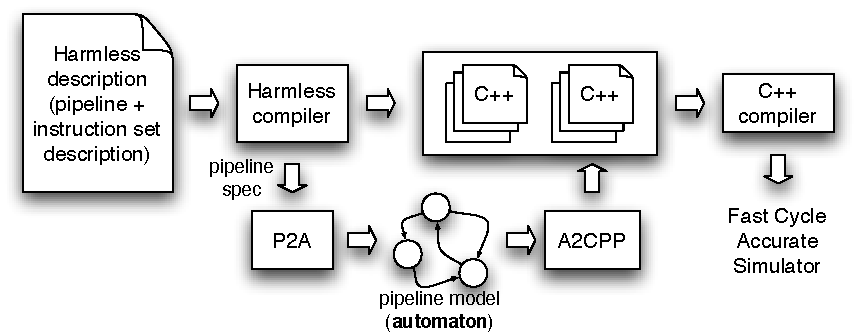
\includegraphics[width=0.8 \linewidth]{../common/images/devTools.pdf}
    \caption{Development chain}
    \label{fig:devTool}
  \end{center}
\end{figure}

These tools are:
\begin{itemize}
\item \gadl\ reads the file description in \harmless. This is the only tool necessary to generate a instruction set simulator (ISS);
\item  \texttt{p2a} and \texttt{a2cpp} are tools that are used for modeling the pipeline, when describing the internal architecture.  A description file of the pipeline is generated by \gadl\ according to the \h\ description,this is the input file of p2a. When the automaton has been generated by p2a, a second tool a2cpp translates the automaton description into $C++$ code, modeling of the pipeline.
\end{itemize}

This documentation focuses on the \gadl\ tool as the integration with the 2 other tools is in early stages of development.

\section{Building \gadl\ from sources}
The build process is made using a python script at the root of the archive : \texttt{buildHarmless.py}. Just configure your Internet access (proxy) if required and run the script. The build script:
\begin{itemize}
\item get the \texttt{galgas} compiler, as \gadl\ is written using the \texttt{galgas} language;
\item build the \texttt{p2a} and \texttt{a2cpp} tools;
\item build the library \texttt{libelf} that will be used to read .elf binary files for the simulators\footnote{\gadl\ is not compatible with the \texttt{libelf} library typically found on Linux distributions (including Ubuntu). Indeed, this library is linked to the simulator generated by \gadl, and we cannot impose a license to the generated code (That is the case with the GNU GPL. We use instead a library under the GNU LGPL. The library can be found on \url{http://www.mr511.de/software/english.html}}.
\end{itemize}

The script does not depends on specific tools (the only specific tools \texttt{galgas} is retrieved from Internet by the script). On Ubuntu/Debian systems, you should only install before basic development tools:
\texttt{apt-get install build-essential}


This script generates one big self-contained binary file that can generate a simulator from a description. The script is tested on Mac OS X, Linux x86/32 bits, Linux x86/64 bits and Linux ARMv6/32 bits. This has not been tested on Windows. 

Please report any problem during install to \url{mailto:harmless@irccyn.ec-nantes.fr}.

\subsection{Description editor}
A syntax file is provided for the \emph{Vim}\footnote{\url{http://www.vim.org}} editor, allowing syntax coloration. You only have to copy the syntax file to \texttt{~/.vim/syntax}. The directory have to be created if it does not yet exist.

With Mac OS X (10.5 required) an XCode project is provided. It can compile directly \gadl, but also build an application (Mac OS X bundle) to edit \harmless\ descriptions. It embeds a text editor with syntax highlighting and \gadl\ compiler.

\section{Dependencies for the simulator generation}

The generated simulator is written in $C++$  and can be used directly, without any dependency. However, a number of dependencies can be added to obtain additional services:
\begin{description}
\item[python] This allows to use the simulator in a Python script, and therefore does not require to recompile the simulator for each new scenario. The open source \texttt{swig}\footnote{\url{www.swig.org}} tool is used to generate the Python wrapper.
\item[libelf] This library allows to read \emph{elf} files, in addition to the default formats (SRecord Motorola and Intel Hex)
\end{description}

This section provides information on how to install these dependencies.

\subsection{Using the simulator with Python}
The simulator is generated in $C++$  and can be used in a Python script (version 2.5 and 2.6 tested). To enable the compilation of the Python wrapper, it is necessary to install the \texttt{Swig} tool:
\begin{itemize}
\item Linux Ubuntu: packages \texttt{swig} and \texttt{python2.5-dev}. The Python interpreter is installed by default.
\item Mac OS X: all is already included in the development tools (10.5).
\item MS Windows: Not tested.
\end{itemize}

\subsection{Library to read ELF files}
\label{sec:elf}
By default, \gadl\ can read the following file formats:
\begin{itemize}
\item Motorola SRecord (SREC)\footnote{\url{http://en.wikipedia.org/wiki/SREC_(file_format)}};
\item Intel Hex\footnote{\url{http://en.wikipedia.org/wiki/Intel_HEX}};
\end{itemize}
To add support for ELF format files \footnote{\url{http://en.wikipedia.org/wiki/Executable_and_Linkable_Format}}, an extra library is required. This last format has the advantage of encapsulating symbols (global variables, functions \ldots) in addition to executable code. 


\emph{Note}: \gadl\ is not compatible with the \texttt{libelf} library typically found on Linux distributions (including Ubuntu). Indeed, the library is linked to the simulator generated by \gadl, and it is not reasonable to impose the generated code to be under a license compatible with the GNU GPL\footnote{\url{http://fr.wikipedia.org/wiki/Licence\_publique\_generale\_GNU}}. We use a library under the GNU LGPL\footnote{\url{http://fr.wikipedia.org/wiki/Licence\_publique\_generale\_limitee\_GNU}}. The library can be found on \url{http://www.mr511.de/software/english.html}. To install it:
\begin{verbatim}
$ ./configure
$ make
$ sudo make install
\end{verbatim}

A local use is preferable on Linux distributions, to prevent conflicts with the other presents.

\emph{Note}: By default, the simulator is generated in 64-bit mode (compiler flag \texttt{-m64}), which gives much better simulation performance. In this case, the library libelf must also support 64-bit:
\begin{verbatim}
$ ./configure
$ make CFLAGS=-m64 LDFLAGS=-m64
$ sudo make install
\end{verbatim}

To stay in 32 bits, you should edit the generated \texttt{Makefile} and remove the \texttt{-m64} flag in \texttt{CFLAGS} and \texttt{LDFLAGS} (or better, update the Makefile.tpl in the template directory).



\section{Generation of a simulator}
The generation of the simulator is from the master file in the case of a description distributed over several files(voir section \ref{sec:plusieursFichiers}).

\gadl\ is a command line tool. Options availables are:
\begin{verbatim}
$ gadl --help
Compiled in 32 bits mode.
Usage : gadl [--help] [--version] [--lexical-analysis-only] [--parse-only] [-v] [--verbose] [--log-file-read] [--no-file-generation] [--Werror] [--detailled-error-messages] [-f] [--message-if-no-format] [-b] [--no-behavior] [-c] [--no-check] [-a] [--no-deasm] [-t] [--no-timing] [-s] [--speed] [-w] [--warn-trunc] [--max-errorss=number] [--max-warningss=number] [--model=string] [--templates=string] file...
Options:
 --help               Display help information
 --version            Display version
 --lexical-analysis-only
                      Perform only lexical analysis on input files
 --parse-only         Parse only input files
 -v,--verbose         Verbose Output
 --log-file-read      Log every file read
 --no-file-generation Do not generate any file
 --Werror             Treat warnings as errors
 --detailled-error-messages
                      Print detailled error messages
 -f,--message-if-no-format
                      get a message when an instruction signature found in a behavior or a syntax part have no corresponding format.
 -b,--no-behavior     does not take into account instruction behavior part. It is not possible to generate an instruction set simulator (ISS)
 -c,--no-check        Remove time consuming checks: orthogonality of instruction set.
 -a,--no-deasm        does not take into account instruction syntax part. It is not possible to generate a dissassembler
 -t,--no-timing       does not take into account instruction timing part. No cycle count. Simulation should be faster.
 -s,--speed           speed option. May be more difficult to debug. Inline component methods.
 -w,--warn-trunc      Warn if the result of an expression may be truncated
 --max-errors=number (default value : 0)
                      Stop after the given number of errors has been reached (by default: 100)
 --max-warnings=number (default value : 0)
                      Stop after the given number of warnings has been reached (by default: 100)
 --model=string       model name that will be generated. By default, all the model defined in the description file are generated.
 --templates=string   Template directory
Handled extension:
 .hadl                a gadl file that can be parsed with an LL1 grammar
\end{verbatim}

For each model described in the description, a directory is created containing the source code of the simulator. Consider for example the description file \texttt{avr.hadl} (included in \gadl\ sources) that contains the model \texttt{AT90CAN128}. The following command:

\begin{verbatim}
$ gadl ./avr.hadl
\end{verbatim}
create the directory  \texttt{./AT90CAN128}, which contains simulator sources. Most important files are:

\begin{verbatim}
Makefile           #file to generate the simulator (requires GNU Make)
arch.h             #main class of the simulator (arch)
arch.i             #C++/Python wrapper file (Swig)
format_all.dot     #describe the tree of the binary description of the instruction set (graphViz)
instConstruct.cpp  #instruction constructor (big file :-/)
instDecoder.cpp    #decode file (related to 'format')
instExec.cpp       #code executed by instructions (related to 'behavior')
instMnemo.cpp      #mnemonic of instructions (related to 'syntax')
instruction.h      #instruction classes
instruction.log    #debug information about the binary part
main.cpp           #simple scenario for the standalone simulator (not used with Python)
main_gdb.cpp       #simulate a gdb-server to use with GNU GDB (not used with Python)
storage.h          #memory model
types.h            #internal data types
\end{verbatim}

\subsection{Compilation options}
\label{sec:cflags}
Different compilation flags are available to modify the simulator behavior:
Main compilation parameters (\texttt{CFLAGS} in \emph{Makefile}) are:
\begin{description}
\item[HOST\_IS\_LITTLE\_ENDIAN] host is \emph{little endian}. This information is required by the \emph{storage} module.
\item[HOST\_IS\_BIG\_ENDIAN] host is \emph{little endian}. This information is required by the \emph{storage} module.
\item[INST\_DECODER\_CACHE\_STATS] This option allows to record memory instruction cache stats (nb of accesses, ratio hit/miss). The simulator speed is slightly altered.
\item[GADL\_NO\_ACTION] This option greatly accelerates the simulation speed. The \emph{action} are used to associate the execution of a piece of code to a memory access (read, write). Actions are used for peripherals description (\texttt{when} keyword). See section \ref{sec:whenReadWrite}.
\item[DEBUG\_MNEMO] To debug syntax part. the internal name of the instruction is printed with the mnemonic.
\item[DEBUG\_STORAGE\_ACCESS] To debug. Each memory access (read or write) is written on stdout. The simulator speed is altered
\item[DO\_NOT\_USE\_INTERNAL\_INSTRUCTION\_CACHE] To debug. Does not use the internal instruction cache associated to the decoder.
\item[DEBUG\_STORAGE\_ADDRESS\_RANGE] To debug. For each memory access, the simulator verifies that the address is in the correct range. Without this option, if an address is our of the memory chunk, a segfault should happen!
\end{description}

The \texttt{Makefile} should be used to generate the simulator (you should have a look to this documented file). Main targets are:
\begin{description}
\item[make standalone] generates a \emph{standalone} simulator. The simulation scenario is contained in the file \texttt{main.cpp};
\item[make python] generates a \emph{python library} of the simulator, see \ref{sec:python}. An example of how to use the python API is included with the AVR example.
\item[make gdb] generates a \emph{gdb server} simulator. This simulator can be used interactively used with gdb, using a UNIX socket. It has been tested successfully with Eclipse and the AVR module. This target works on POSIX hosts (Linux, Mac OS X).
\item[make clean] remove generated files.
\end{description}


\section{Using the simulator}
The API is available both for $C$/$C++$ and Python (through the SWIG wrapper).

The main $C++$ object is \texttt{arch} that should be used to have an instance of the processor.

Following sub-sections give main functions to deal with the simulator.
\subsection{System Observation}

\paragraph{\texttt{void decoderStats()}}
The method displays information on the internal decoder cache (used to speed up simulation). This command is valid only if the cache is used to decode (no option \texttt{DO\_NOT\_USE\_INTERNAL\_INSTRUCTION\_CACHE}) and if statistics are allowed (\texttt{INST\_DECODER\_CACHE\_STATS}), see section \ref{sec:cflags}:
\begin{verbatim}
Internal decoder instruction cache Ratio
    12128 accesses.
    Miss : 1217
    Hit : 10911
    Hit Ratio : 0.899654
    cache contains : 524 instructions
    (capacity is 1024 instructions)
    cache use ratio : 0.511719
\end{verbatim}

\paragraph{\texttt{unsigned int const getNBCycles()}} give the number of cycles since the beginning of the simulation. This is not used in the ISS mode (Instruction Set Simulation).
\paragraph{\texttt{unsigned int const getNBInstructions()}} give the number of instruction executed since the beginning of the simulation.
\paragraph{\texttt{string disassemble(const unsigned int ipStart, const int nbBytes, bool verbose)}} disassemble code from address
\texttt{ipStart}, for \texttt{nbBytes} bytes. If \texttt{verbose} is \texttt{true}, The decoding address and the instruction binary code are displayed.

\subsection{Execution}
\paragraph{\texttt{void reset()}}
At this date, it only reset the program counter.

\paragraph{\texttt{void execInst(const unsigned int nb)}} Execute \emph{a maximum of} \texttt{nb} instructions, either in CAS (Cycle Accurate Simulation) or ISS (Instruciton Set Simulation). If breakpoints are used, it should stop before.

\paragraph{\texttt{void runUntil(const unsigned int addr, const unsigned int max)}} simulate until the program counter is  \texttt{addr}. The simulator executes \emph{a maximum of} \texttt{max} instructions. If breakpoints are available, they are more efficient (no test at each clock cycle).

\paragraph{\texttt{bool readCodeFile(const char *filename, const bool verbose = false)}} read a binary code file and put it into the memory. Valid formats are: SRecord, Intel Hex or .elf, voir section \ref{sec:elf}). An error is generated if the file format is not recognized. Only memory section with \texttt{program} in the \h\ description of the memory can get program code (see section \ref{sec:mem_program}).

\subsubsection{Breakpoints}
Using breakpoints requires the \emph{actions} (execution of a piece of code related to a memory access (read, write or execute). Compilation flag \texttt{USE\_INTERACTIVE\_SIMULATION} should be set, and \texttt{GADL\_NO\_ACTION} should \emph{not} be set. see section \ref{sec:cflags}.
\paragraph{\texttt{void addBreakpoint(const unsigned int addr)}} Add a breakpoint for interactive simulation. An error is generated if there is already a breakpoint.
\paragraph{\texttt{void addBreakpoint(const char *symbolName)}} Add a breakpoint using the symbol name instead of the address (if symbols are available, with ELF files).
\paragraph{\texttt{void removeAllBreakpoints()}} 
\paragraph{\texttt{void removeBreakpoint(const unsigned int addr)}} Remove breakpoint at the specified address. An error is generated if there is not breakpoint.
\paragraph{\texttt{void removeBreakpoint(const char *symbolName)}} remove a breakpoint using symbol name instead of address.

\paragraph{\texttt{storage * getProgramChunk(const unsigned int address)}} Allow to get the memory chunk related to an address. This allows to read or write data in memory (see \texttt{storage.h} for further details).
\paragraph{\texttt{void setProgramCounter(u32 val)}} Define the value of the program counter (independently of the name used in the description (IP, PC,  \ldots).

\paragraph{\texttt{u32 programCounter()}} Read the value of the program counter (independently of the name used in the description (IP, PC,  \ldots).

\subsection{Symbols}
Using symbols instead of memory addresses is available only for .ELF files (see section \ref{sec:elf}).

\paragraph{\texttt{bool getSymbolObjectAddress(const char *symbolName, u32 \&v\_addr, u32 \&size)}} Search for the virtual address and size of the symbol name. It returns true if a symbol have been found, and updates \texttt{v\_addr} and \texttt{size}
\paragraph{\texttt{bool getFunctionName(const char *symbolName, u32 \&v\_addr)}} Search for the virtual address and size of the symbol name. It returns true if a symbol have been found, and updates \texttt{v\_addr}

\paragraph{\texttt{u32 getPhysicalAddress(const u32 v\_addr, bool \&found)}}  allows to get the physical address from the virtual one. \texttt{found} is set to \texttt{false} if the value is not in any available range.

it is easier to pool the common description of instructions

\subsection{Using Python}
\label{sec:python}
The main advantage of using Python to run scenarios is that it is no more necessary to recompile the simulator for each new scenario. When compiling the harmless simulator, a wrapper is generated with swig and a python module is built. In Python, it is then possible to call any C methods defined in the first part of this section.

For example, consider the AVR simulator provided in the examples directory. The model is called \texttt{AT90CAN128}, which is the name of the module to call. The following script calculates the number of instructions between 2 access to the function \texttt{function\_of\_task\_startTask}, 10 times:

\lstset{language=Python}
\begin{lstlisting}
#!/usr/bin/python
from AT90CAN128 import arch

f=arch()
f.readCodeFile("../trampoline.elf")
f.addBreakpoint("function_of_task_startTask")
nbInst = 0
f.printRegs()
for i in range(10):
    f.execInst(10000000) #run until breakpoint
    print f.getNBInstructions() - nbInst,  " insts between 2 breakpoints"
    nbInst = f.getNBInstructions()
f.printRegs()
f.decoderStats()
\end{lstlisting}
\lstset{language=Harmless}

\part{Description of the Instruction Set} 
%!TEX root = ./main.tex
%!TEX encoding = UTF-8 Unicode
\chapter{Modeling the Instruction Set}
\section{Modeling using 3 views}
\label{sec:modelisationArborescente}
\subsection{Tree modeling approach}
\harmless\ uses 3 views to describe the instruction set of a processor:
\begin{itemize}
\item the binary view (\emph{format}) is used to describe the binary format of instruction to enable the decoding stage of instructions
\item the behavioral view (\emph{behavior}) allows to describe the behavior of instructions to simulate instructions.
\item the syntax view (\emph{syntax}) allows to describe the mnemonic of instruction to generate the disassembler.
\end{itemize}

Each view is a set of tree where each node describes a portion of \emph{format}, \emph{behavior} or \emph{syntax}. The description of a node is as follows:
\begin{verbatim}
<kind> <name> <kind_options>
  <kind_body>
end <kind>
\end{verbatim}
where \texttt{<kind>} can be \texttt{format}, \texttt{behavior} or \texttt{syntax}. By default, a node aggregates the sub nodes which are defined in the body. However, using the keyword \texttt{select}, a node may be chosen among others in the description of each trees.

This tree approach aims to factor up similar items (for the syntax, behavior or binary format). In each view, an instruction is represented by a branch in a tree. Instructions that share certain characteristics in a view share the same nodes.

\subsection{Instruction identification}
\label{sec:signature}
A node can have one or more \emph{tags}. A tag is represented in  \harmless\ using the \texttt{\#} character, followed by an alphanumerical string.
The \emph{set} of \emph{tags} along a branch of a tree is the unique identifier of an instruction and is called the \texttt{Instruction Identification.} The identification is a \emph{set}, which means that there is no order and no counting of the number of occurrence of each tags.

In some cases, it is useful to \emph{mark} tags, because the same node can be used in different contexts. For instance, when reading 2 source registers and one destination register, we use \emph{extended-tags}. An \emph{extended-tag} is represented using the \texttt{@} character, followed by an alphanumerical character string. As a consequence, each tags in the subtree are modified by adding the \emph{extended-tag} as a suffix (without the \texttt{@} character).

This mechanism is used to link instruction between the different views (format, syntax and behavior).

\subsection{An example}
\label{exempleSignature}
More detailled examples are given in the chapters associated to each views. The goal here is to show how is described the tree structure.
Consider for example the following (simplified) code:

\begin{lstlisting}
behavior readGPR #read8
  ...
end behavior

behavior writeGPR #write8
  ...
end behavior

-- instruction that operate on 2 source registers
behavior twoRegsOp
  -- read the 2 source registers
  readGPR@src1
  readGPR@src2
  select
    case #ADC  ...
    case #ADD  ...
    case #SUB  ...
  end select
  writeGPR
end behavior
\end{lstlisting}
This example describe 3 \texttt{behavior} nodes (non terminal):  \texttt{readGPR}, \texttt{writeGPR}, and \texttt{twoRegsOp}. The node \texttt{twoRegsOp} is the root, because it is not called by any other node. 

\begin{figure}		%% Small Example
  \begin{center}
    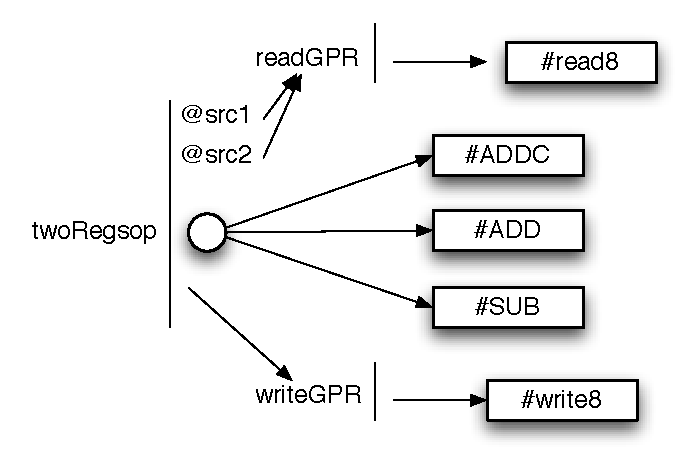
\includegraphics[width=0.8 \linewidth]{../common/images/instBase.pdf}
    \caption{Tree representation of the simple example.}
    \label{fig:instBase}
  \end{center}
\end{figure}

It is graphically represented in figure \ref{fig:instBase}. Each node is represented by name and by a vertical bar. To the right of the vertical bar, the various "elements" (selection, call for another node with or without \emph{extended-tag}) are shown \emph{sequentially}. The circle represent the structure of selection (\texttt{select}). Tags are represented in rectangles, and extended-tegs are represented in the calling node.

The advantage of using one extended-tag here lies in the fact that the \texttt{readGPR} node is called in 2 different contexts: one for each source register. As the extended-tag is added to each tags in the subtree, there are differentiated: \texttt{\#read8src1} and \texttt{\#read8src2}.

So in this example, the ADD instruction as a set of tags:  \texttt{\#read8src1}, \texttt{\#read8src2}, \texttt{\#ADD} and \texttt{\#write8}.
Similarly, the SUB instruction as a set of tags: \texttt{\#read8src1}, \texttt{\#read8src2}, \texttt{\#SUB} and \texttt{\#write8}. These set of tags represent the \emph{instruction identification}.

In the internal representation, each instruction is modeled using a $C++$ class, where the name of the class is here  \texttt{cpu\_ADD\_read8src1\_read8src2\_write8}. To define the internal name of an instruction, the name of the model (here \texttt{cpu} is concatenated with the set of tags in the alphabetical order, separated by the '\texttt{\_}' character.

%\subsection{Intérêt de la structure selon 3 vues}
%TODO 

%!TEX root = ./main.tex
%!TEX encoding = UTF-8 Unicode
\chapter{Fundamentals of language}
\section{Lexical Elements}
This section lists all lexical elements which are used by \harmless. Spaces and indentations are ignored by the lexical analyzer (as in C): indentation has no influence on the language, although it facilitates the reading!
As many instructions look very much like the $C$ language, the $;$ character is understood as a space.

\subsection{Comments}
\label{sec:commentaire}
Comments use the same syntax as in VHDL. They begin with \texttt{--} and ends at the end of the line.

\begin{lstlisting}
--  This is a comment
\end{lstlisting}

\subsection{Character String}
\label{sec:chaines}
A string is represented using double quotes \texttt{"} (like in $C$):
\begin{lstlisting}
"This is a character string"
\end{lstlisting}
Carriage returns are ignored.

\subsection{Integers}
\label{sec:nombres}
Integers can be written with different bases: binary, decimal, octal and hexadecimal, preceding the number by respectively \texttt{\bs b}, \texttt{\bs d}, \texttt{\bs o} and \texttt{\bs x}. Decimal format is used by default:
\begin{lstlisting}
38    -- 38 (decimal)
\d12  -- 12 (decimal -> default)
\b100 -- 4 (binary)
\o70  -- 56 (octal)
\x2F  -- 47 (hexadecimal)
\end{lstlisting}

The \texttt{s} character is used as a suffix for \emph{signed integers}.
\begin{lstlisting}
38  -- unsigned integer -> 6 bits
38s -- signed integer   -> 7 bits
\end{lstlisting}

To help readability, the \texttt{\_} character can be added everywhere in the integer definition, it will be deleted by \harmless\ during lexical analysis:
\begin{lstlisting}
\b1001_1111 -- 9F hexa
\end{lstlisting}

Finally, it is possible to add the suffix \texttt{kb} ($2^{10}$=1024 bytes) and \texttt{mb} ($2^{20}$= 1048576 bytes). It is useful for address space definition:
\begin{lstlisting}
128kb -- equivalent to 131 072
4mb   -- equivalent to 4194304
\end{lstlisting}

\subsection{Mask}
\label{masque}
A mask allows to express a set value depending on the value of different bits. The masks are only values coded as binary:
\begin{lstlisting}
\m11-0 -- correspond to 1110 or 1100
\end{lstlisting}
A mask is prefixed by \texttt{\bs m}. The binary number is expressed by \texttt{0}, \texttt{1} and \texttt{-}, the latter indicating that the value of the corresponding bit is not useful. 

Masking operations are mainly used for decoding instructions (see Chapter \ref{chap:format}).

\subsection{Floats} 
There is currently no support for floating point numbers in Harmless.

\subsection{Keywords}
\label{keywords}
Reserved keywords for the language are:
\begin{lstlisting}
model, port, device, architecture, write, shared, behavior, format, select, error, warning, component, void, every, memory, width, address, type, RAM, ROM, register, stride, read, program, counter, pipeline, stage, init, run, as, machine, BPU, bypass, release, in, maps, to, default, instruction, fetch, debug, big, little, endian, except, do, out, when, on, field, nop, slice, case, is, others, signed, or, syntax, switch, number, octal, decimal, hexadecimal, binary, suffix, prefix, return, print, if, then, elseif, else, loop, while, end, true, false, ror, rol, cat, timing, decode, size, jumpTaken, add, cycle, use, interrupt
\end{lstlisting}

\subsection{Delimiters}
Delimiters are mostly used for expressions and assignments:
\begin{lstlisting}
: .. . , {   } [ ] :=  ( ) !  ~  * /  %  + - <<  >>  < >  <=   >=  
=  !=  &  ^  |  &&  ^^  ||;
\end{lstlisting}

\subsection{Tags}
\label{sec:etiquettes}
Tags are used to enable a correspondence between different views of an instruction (behavior, binary and syntax). An instruction is then modeled as a set of tags, which form its \emph{signature} (see chapter \ref{sec:signature}).

\emph{Tags} begins with character \texttt{\#}, followed by alphanumerical characters (\texttt{a..z}, \texttt{A..Z}, \texttt{0..9}, \texttt{\_}).

In few cases, we use an \emph{extended tag}, which is a tag that will be added for each node called. An \emph{extended tag} begins with character \texttt{\@}, followed by alphanumerical characters (\texttt{a..z}, \texttt{A..Z}, \texttt{0..9}, \texttt{\_}).

\subsection{Identifier}
\label{sec:identifiant}
An identifier is an alphanumerical characters string (\texttt{a..z}, \texttt{A..Z}, \texttt{0..9}, \texttt{\_}) where the first letter is not a number. It cannot be a keyword, nor a data type (\texttt{u} or \texttt{s} followed by a number), see section \ref{sec:TypeDonnees}.

\section{Data types}
\label{sec:TypeDonnees}
At this date, \harmless\ can only handle integer data types. Data may be signed or unsigned, and size is defined at the bit level. Data types are defined using  \texttt{s} (signed) or \texttt{u} (unsigned) characters, followed by a number which define the size of the data in bits:
\begin{lstlisting}
u17 val1 --  val1 is an unsigned 17 bits value
s9 val2  --  val2 is a signed 9 bits value
u1 bool  -- u1 is understood as a boolean value.
\end{lstlisting}
Internal implementation limits sizes to 64 bits at this date, because these types are directly mapped on $C$ types.

An immediat value has the minimal size required to be coded:
\begin{lstlisting}
38  -- unsigned integer -> 6 bits -> u6
38s -- signed integer -> 7 bits -> s7
-1s -- signed integer -> 2 bits -> s2
\end{lstlisting}

\section{Cast}

The \emph{cast} allows to change the type of a value. A sign extension is performed when casting \emph{to a signed type} (and \emph{only} to a sign type. Examples:
\begin{lstlisting}
(s8)(-1s)  -- cast a s2 (signed with 2 bits) to a s8: result is 0xFF
(u32)(-1s) -- cast a s2 to a u32 (no sign extension!): result is 0x03
(u32)((s32)(-1s)) -- cast a s2 to a s32 (sign extension) and to u32
\end{lstlisting}


%\begin{verbatim}
\section{Expressions}
\label{sec:expressions}
Expressions are largely inspired by the $C$ language, with some extensions for bit manipulations. We found the following $C$ operators: $($, $)$, $!$, $\sim$, $*$, $/$, $\%$,$+$, $-$, $<<$, $>>$, $<$, $>$, $<=$, $>=$, $=$, $!=$, $\&$, $\wedge$, $|$, $\&\&$, $||$.

Note, however, even if these expressions are slightly the same as in $C$, there are differences on the size of values returned. See \ref{sec: typeExp}

Expression enhancements are about type casts, rotations, concatenation and access to bit fields, these operation are not available in $C$.

\subsection{Expressions Priorities}
All expressions sorted by priority are defined in Table \ref{tab:exp}.

\begin{table}[!h]
\begin{center}
\begin{tabularx}{\columnwidth}{|c|c|X|}
\hline
\bf expression & \bf priority & \bf use  \\  \hline
idf & 1 & variable, register, memory access. Call to a component's method ... \\ \hline
idf[index] & 1 & access to a tabular value \\ \hline
nombre & 1 & numerical value (signed or not). \\ \hline
(exp) & 1 & parentheses\\ \hline
(type)(exp) & 1 & cast expression 'exp'. Unlike the $C$, parentheses are required, in order to eliminate This expression ambiguity \\ \hline
\{field\} & 2 & Access to a bit field. See \ref{sec:field} \\ \hline
 ! & 3 &  Logical not: returns \emph{true} or \emph{false} \\ \hline
$\sim$  & 3 & bitwise not \\ \hline
-  & 3 & unary minus \\ \hline
* / \%  & 4 & multiplication, division, modulo \\ \hline
+ -  & 5 & Addition, subtraction \\ \hline
$<<$ $>>$ & 6 & left and right shift (as in $C$)\\ \hline
ror rol & 6 & right and left rotation: \texttt{exp rol 3} rotate bits of \emph{exp} 3 bits to the left \\ \hline
$<$ $>$ $<=$ $>=$ & 7 & logical comparison \\ \hline
$=$ $!=$  & 7 & equal logic \\ \hline
$\&$  & 8 & bitwise and \\ \hline
$\wedge$  & 9 & bitwise xor \\ \hline
$|$   & 10 & bitwise or \\ \hline
$\&\&$  & 11 & logical and \\ \hline
$||$   & 12 & logical or \\ \hline
cat   & 13 & concatenation of expressions \\ \hline
\end{tabularx}
\caption{Expressions evaluation priorities in \harmless (1 being the highest priority)}
\label{tab:exp}
\end{center}
\end{table}

%TODO: exemple pour ror/rol, cast et cat.

\subsection{Result type expressions}
\label{sec:typeExp}
The type of an expression is strong. It is not based solely on the size of the input data, but also on operations that are performed on it. For example:
\begin{itemize}
\item adding 2 numbers of $n$ and $m$ bits returns a result of $max(n,m)+1$ bits;
\item multiplication of 2 numbers of $n$ et $m$ bits returns a result of $n+m$ bits;
\item shifting $d$ bits left a value of $n$ bits returns a result of $n+d$ bits;
\item shifting $d$ bits left a value of $n$ bits returns a result of $n-d$ bits;;
\end{itemize}
%TODO: pas fini.

\subsection{Bitfield access}
\label{sec:field}
The access to a field is using braces. The definition of a field by setting the most significant bit first, followed by '\texttt{..}' and the lowest bit. The second value must be lower than the first.

\emph{In \harmless, the LSB has always the index 0}. The MSB has index 'size of data' - 1. 
This is notably not the case with some manufacturers documentation indicating the bit 0 as the most significant bit (PowerPC, for example).If a single bit is used, the second part is not required. Several fields can be defined, separated by commas:
\begin{lstlisting}
u8 val1 --  val1 is unsigned 8 bits
 -- val2 gets the 4 lowest significant bits of val1
u4 val2 := val1{3..0}
--  val3 gets bit 4, concatenated with the 2 lowest significant bits of val1.
u3 val3 := val1{4, 1..0}
u8 val4 := 3;
-- we can use expressions to define a field.
u2 val5 := val1{val4+1..val4}
\end{lstlisting}

You can also use an expression to define an element of a field, but this expression must return an \emph{unsigned} value. Expressions can not be allowed in certain cases (format definition), because \harmless is not always able to extract the size of the field.

\section{Instructions}
language instructions are used in a limited area for implementation: in a \emph{do}..\emph{end do} when defining behavior or in the definition of a component, ...

There are no instruction for loops at this date, even if a statement will be added in the short term (the instruction type \emph{store multiple word} of the PowerPC, for example).

Following statement are provided:
\subsection{Assignment}
assignment use the operator \texttt{:=}, to avoid ambiguity with a comparison: \texttt{<variable> :=  <expression>}:
\begin{lstlisting}
val2 := val1{3..0} -- val2 gets the 4 lowest significant bits of val1
\end{lstlisting}

It is allowed to use bitfields in the left part of an assignment (see \ref{sec:field}):
\begin{lstlisting}
u8 val2;
-- assign the 4 most significant bits of val2
-- the 4 loewt significant bits are not modified.
val2{7..4} := val1{3..0}
\end{lstlisting}

\subsection{Conditional statement}
The conditional statement has the form: \texttt{if <expresssion> then <implementation> [elseif <implementation>] [else <implementation>] end if}
\begin{lstlisting}
u16 newPC;
if CCR{bitIndex} = 0 then 
  newPC := (u16)((s16)(PC)+k) 
else 
  newPC := (u16)(PC)
end if 
\end{lstlisting}

\subsection{Loops}
Loops have the form: \texttt{loop <guard> while <condition> do <implementation> end loop}. \texttt{Guard} is the maximal number of iterations allowed, due to prevent infinite loops. The algorithm used by the simulator is:
\begin{lstlisting}
u64 loop = 0;
while(loop < guard && condition)
  loop = loop + 1;
  <implementation>
if(loop == guard)
  -- send runtime error.
\end{lstlisting}

\emph{Loops are allowed in an \harmless\ description only to generate an instruction set simulator. There are many restrictions with CAS.}

Loops may be used to model instructions when the algorithm is based on a loop, but the hardware implementation does not need such mechanism. This is the case for instance of the ARM instruction CLZ (\emph{Count Leading Zeroes} that counts the number of zeros, from the MSB. For this instruction, we may use the following code:
\begin{lstlisting}
u6 clz(u32 value)
{
  u1 found := false
  u6 currentBit := 32
  loop 32 
  while (!found && currentBit != 0) do
    if value{currentBit-1} then 
      found := true
    else
      currentBit := currentBit - 1
    end if
  end loop
  return 32 - currentBit
}
\end{lstlisting}
The guard limits the loop to 32 iterations.

\emph{In the case of instructions where the implementation is based on a loop (\emph{Load/Store Multiple Word} for PowerPC and ARM instruction sets), the generated CAS does not take into account multiple access to methods (access only one time).}

\subsection{Return statement}
This statement can return a comma separated list of values within a method component(section \ref{sec:component}), the same approach as C. This statement is not always available (for example in the implementation of a \emph{behavior}).

The form is: \texttt{return <expression1>,<expression2>, \ldots}:
\begin{lstlisting}
return val1,val2
\end{lstlisting}

\subsection{Nop statement}
This instruction can inhibit xx next instructions. It is a feature found on some processors such as Atmel AVR. This instruction is available on the implementation part of a  \texttt{behavior}.

The form is: \texttt{nop <expression> instruction}
\begin{lstlisting}
-- the next instruction won't be executed.
nop 1 instruction
\end{lstlisting}

\subsection{Error statement}
\label{sec:instError}
These instructions allow to generate run-time error or a warning on an abnormal state of the simulator.

Some devices can be partially described: a \emph{timer/counter} with only the model of the \emph{timer} part, prohibited combinations from documentation, \ldots. These cases can be detected by the simulator. 

The form is: \texttt{error <character string>} or \texttt{warning <character string>}. 
At this date, only the error string is printed on \texttt{stderr} at run-time.

\begin{lstlisting}
warning "error message"
\end{lstlisting}

At run-time, the following message will be printed on \texttt{stderr}: 
\texttt{RUNTIME WARNING at file '/Users/mik/../avr.hadl', line 54:30. Message is "error message"}

\subsection{Display statement}
This instruction allows you to write a string on the error output (stderr). This is particularly useful to model peripherals: \\
\texttt{print (<expression>|<characterStr>)[,(<expression>|<characterStr>)][, ...} 

For a serial port: 
\begin{lstlisting}
print UDR0
\end{lstlisting}
Will print the value of the register \texttt{UDR0} on stderr. The value will be interpretated has in $C$ (ASCII for a value of 8 bits or less), numerical value in other cases (hex).

For a GPIO:
\begin{lstlisting}
print "port A: ",PORTA,"\n"
\end{lstlisting}

\subsection{Interrupt}
\label{keyword:interrupt}
Interrupt hardware management is described in chapter \ref{chap:interrupt}. The \texttt{interrupt} keyword allows to set an interrupt. 
The form is: \texttt{interrupt <unsigned number>}, where the unsigned number is the \texttt{id} of the interrupt.
\begin{lstlisting}
interrupt 5
\end{lstlisting}
This value will be available for the hardware interrupt handler.

\section{Organization of a description}
A description follows the general schema:
\begin{verbatim}
<modelDeclaration> 
repeat 
  while <inModel>; 
  while <default>; 
  while <component>; 
  while <pipeline>; 
  while <machine>; 
  while <architecture>; 
  while <format>; 
  while <behavior>; 
  while <syntax>; 
  while <timing>; 
  while <printNumberType>; 
end repeat;
\end{verbatim}
The structure \texttt{repeat..while..end repeat} indicates that it is possible to put each of these rules in any order as many times as needed (even 0).
The parts are:
\begin{itemize}
\item \texttt{modelDeclaration} identifies the model. It is possible to declare many models in the same description, see section \ref{sec:plusieursModeles};
\item \texttt{inModel} is used when describing many models, see section \ref{sec:plusieursModeles};
\item \texttt{default} allows to define default parameters. It is mandatory and defined in section \ref{sec:default};
\item \texttt{component}  describe an hardware \emph{component}, see section \ref{sec:composant};
\item \texttt{format} \texttt{behavior} and \texttt{syntax} are related to the instruction set description (3 views), see \ref{chap:format},  \ref{chap:behavior} and  \ref{chap:syntax};
\item \texttt{printNumberType} is used in syntax description, see \ref{chap:syntax};
\item \texttt{timing} is used in a temporal description, without taking into account the underlying micro-architecture;
\item \texttt{pipeline} \texttt{machine} and \texttt{architecture} are used for the description of the micro-architecture.
\end{itemize}
No order of the different part is required.

\subsection{Dealing with multiple description files}
\label{sec:plusieursFichiers}
The description of a processor can use multiple files, which are then used to generate a simulator. 
For example, the instruction set of the PowerPC can be described in a first file \texttt{powerpc\_instSet.hadl} which is then used in the description of different models (\texttt{5516}, \texttt{565}, \texttt{750}, \texttt{970}, ...):
\begin{lstlisting}
include "powerpc_instSet.hadl"
\end{lstlisting}
Currently, no verification is performed to detect cyclic inclusions.

%section "défaut."
\subsection{\emph{Default} section}
\label{sec:default}
The \texttt{default} section is mandatory and set some global settings.
\subsubsection{default size of instructions}
This parameter gives the basic size of instructions for decoding. For example, all of the PowerPC instructions are 32 bits wide, so the value should be set to 32, but with the HCS12, where instruction sizes are from 1 to 8 bytes, the value is 8:
\begin{lstlisting}
default {
  instruction := 8
}
\end{lstlisting}
This parameter is used in the decode phase.

\subsubsection{Endianness}
The endianness should be given (used when accessing memory):
\begin{lstlisting}
default {
  big endian
}
\end{lstlisting}
or \texttt{little endian} when using the lowest significant byte first.
\emph{At this date, it's not possible to change endianness dynamically.}
This parameter is mandatory.

\section{Description of several models in the same file}
\label{sec:plusieursModeles}
This approach is used to describe different variants of an architecture.
The declaration of the different models is:
\begin{lstlisting}
model mod1, mod2, mod3 
{
\end{lstlisting}
In this example, the file contains 3 models \texttt{mod1} to \texttt{mod3}. In the generation process, directories \texttt{mod1/} to \texttt{mod3/} will be created, each one having the sources of one simulator.

The description is common to all the models by default. To get a specific part, the following command should be used:
\begin{lstlisting}
-- the description between {} is valid
-- only for mod1 and mod2:
in mod1, mod2 {  bla bla bla }
\end{lstlisting}
the \texttt{*} is similar to 'every models', and the keyword \texttt{except} is used to remove particular models
\begin{lstlisting}
-- identical to the previous description.
in * except mod3 { 
\end{lstlisting}

The granularity of the \texttt{in} keyword is restricted to high level elemets: a whole component, a \texttt{behavior}, a \texttt{format}, \ldots

%!TEX root = ./main.tex
%!TEX encoding = UTF-8 Unicode
\chapter{Description of instructions binary code}
\label{chap:format}
The description of the instruction format is based on a tree structure, allowing up to pool the common format of each instruction. The objective here is to extract from the binary format of instruction, both the type of instruction, and the operands. In the generated simulator, this step takes place in the \emph{decoding} phase of instructions.

We will study in a first approach fixed size instruction set. The description will then be extended to variable size instruction sets in section \ref{sec:formatTailleVariable}.

\section{General architecture}
The description of the binary format will allow to decode the binary format of instructions. Initially, it is necessary to provide in section \texttt{default} the basic size of instructions:
\begin{lstlisting}
default {
    instruction := 16  -- default instruction size in bits
}

\end{lstlisting}
In this example for instance, the instruction size is 2 bytes or a multiple of 2 bytes for the variable-size instruction sets. For example, instructions sizes in the \texttt{HCS12} are from 1 to 8 bytes. In this case, you should specify \texttt{instruction := 8}.

The description of the format describes how to decode the binary word whose size is supplied.

The general structure of the description of format nodes is:
\begin{lstlisting}
format <name> [tag]
  <formatBody>
end format
\end{lstlisting}

\texttt{<formatBody>} is a sequence of elements:
\begin{itemize}
\item \emph{tags};
\item call to another format
\item select structure, using the \texttt{select} keyword. See section \ref{sec:formatSelect};
\item definition of operands. See section \ref{sec:operandeFormat}.
\end{itemize}

\subsection{Select structure}
\label{sec:formatSelect}
The \texttt{select} statement allow to differentiate different branches of the tree, like in the description of each view.

The select statement acts on a bit field of the binary format of the instruction:
\begin{lstlisting}
  select slice <field>
    case <masque> is <formatBody>
    case .. 
  end select
\end{lstlisting}

\subsubsection{\texttt{field} part}
The \texttt{field} part indicate the binary part of the instruction code that will be used to differentiate instructions. For example, let's consider instructions \texttt{ADDC} and \texttt{ADD} of AVR, where the binary representation is given in figure \ref{fig:selectFormat1}.

\begin{figure}[h]		%% select sur ADD et ADDC
  \begin{center}
    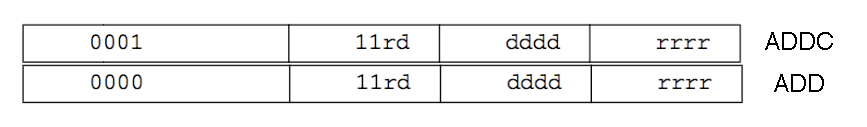
\includegraphics[width=0.8 \linewidth]{../common/images/selectFormat1.pdf}
    \caption{Binary code of instructions \texttt{ADDC} and \texttt{ADD} of Atmel AVR® (code size is 16 bits).}
    \label{fig:selectFormat1}
  \end{center}
\end{figure}

In this case,the following construction can be used:
\begin{lstlisting}
  select slice {12}
    case 0 is ... -- ADC
    case 1 is ... -- ADD
  end select
\end{lstlisting}

Indeed, only bit 12 distinguishes the 2 instructions. The \texttt{<field>} part is written in the same way than a bitfield of a variable (section \ref{sec:field}), but only numerical values can be used (no expressions):
\begin{lstlisting}
  select slice {12..10, 3..2} -- select bits 12 to 10 and 3 to 2 (5 bits selected)
\end{lstlisting}
The  \texttt{<field>} part size should be guessed statically.

\subsubsection{\texttt{mask} part}
The \texttt{mask} part operates on bit fields taken from the \texttt{field} part. It could not have a higher size than the \texttt{field} one (an error is generated during generation of the simulator).

The \texttt{mask} part can be either a numerical value (as in the previous example) or a binary mask (see section \ref{masque}). When using a binary mask, charater \texttt{-} can either be understood as a \texttt{0} or \texttt{1}. Using the example of figure \ref{fig:selectFormat1}, if we want to pool the common part of the 2 instructions:
\begin{lstlisting}
  select slice {15..10}
    case \m000-11 is .. -- both ADD and ADDC
    case ...
  end select
\end{lstlisting}
In this case, a selection is done on the whole \emph{opcode} (binary code except the operands). The first \texttt{case} will be taken only if bits \texttt{15..10} are \texttt{000011} (\texttt{ADD}) or \texttt{000111} (\texttt{ADDC}).

The \texttt{or} operator allow to select different mask for one case:
\begin{lstlisting}
select slice {7..0}
    case \x1B or \x1A or \x19 is ...
    ..
\end{lstlisting}
This example, extracted from the description of the Freescale \emph{HCS12}, allow to pool different cases, although their correspondence at the binary level is not possible.

Eventually, all the other case may be pooled using the \texttt{others} keyword.
\begin{lstlisting}
  select slice {2..0}
    case \m110 is ...
    case \m111 is ...
    others     is ...
  end select
\end{lstlisting}
In this example, the last choice will be taken for all formats that not match \texttt{11-}.

The \texttt{others} keyword can only be used one time in a \texttt{select} statement, and it should be the last case.

\subsubsection{\texttt{<formatBody>} part}
The \texttt{<formatBody>} is the body of a \emph{format} node.

\subsection{Extracting operands}
\label{sec:operandeFormat}
The extraction of operands use the \texttt{slice} keyword, with a bitfield. Given the 2 instructions \texttt{ADD} and \texttt{ADDC} in figure \ref{fig:selectFormat1}:
\begin{lstlisting}
  r := slice{9, 4..0} -- size: 5 bits
  d := slice{8..4}    -- size: 5 bits
\end{lstlisting}
Size of operands is computed statically. In other views (\emph{behavior} and \emph{syntax}), operands values can be retrieved as constant. In that case, the \texttt{field} keyword is used:
\begin{lstlisting}
  field u5 r
  field u5 d
\end{lstlisting}

Some operands need to be declared as signed values (for a branch for example). This is done using the \texttt{signed} keyword:
\begin{lstlisting}
  k := signed slice{11..0}
\end{lstlisting}
\texttt{k} type is \texttt{s12}.

Eventually, it may be useful to operates directly on the operands. A shift operator is provided (limited to a numerical value):

\begin{lstlisting}
  RdIndex := slice{7..4} << 1
\end{lstlisting}
In that case, \texttt{RdIndex} type is \texttt{u5}.

\section{Example}

This example is based on a part of the XGate instruction set. XGate is a co-processor integrated in the \emph{HCS12X}. It is based on a RISC architecture, with a 16 bits, fixed sized, instruction set. 16 GPR (8 bits) are provided.

\subsection{Description of a part of the instruction set of XGate}
Figure \ref{fig:shiftAndTriadicInstFormat} gives the binary format of shift and triadic instructions.

\begin{figure}[h]		%% select sur ADD et ADDC
  \begin{center}
    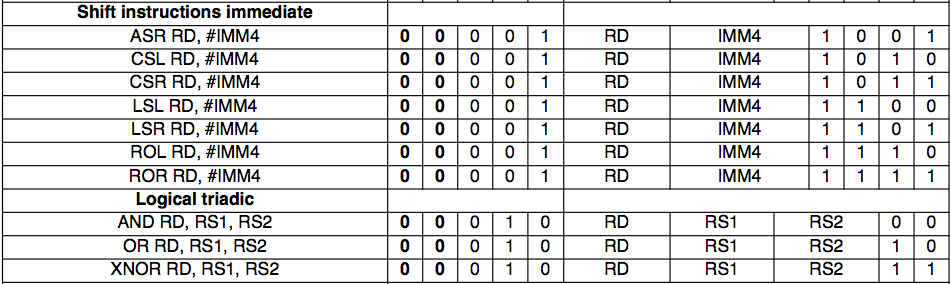
\includegraphics[width=0.95 \linewidth]{../common/images/shiftAndTriadicInstFormat.png}
    \caption{Binary code of shift and triadic instructions of XGate® \emph{Source Freescale}}
    \label{fig:shiftAndTriadicInstFormat}
  \end{center}
\end{figure}

We can directly note on this example that the bit 12 serves to differentiate the 2 types of instructions. More generally for the whole instruction set, the 5 most significant bits allow to identify instruction families (\emph{opcode}):
\begin{lstlisting}
format inst
  select slice {15..11}
    case \b00001 is shiftInstructionImm
    case \b00010 is logicalTriadic
  end select
end format
\end{lstlisting}
For shift instructions, the \texttt{shiftInstructionImm} format node is used:
\begin{lstlisting}[firstnumber=7]
format shiftInstructionImm #IMM
  rdIndex := slice{10..8}
  imm4 := slice{7..4}
  select slice {3..0}
    case \b1001 is #ASR
    case \b1010 is #CSL
    case \b1011 is #CSR
    case \b1100 is #LSL
    case \b1101 is #LSR
    case \b1110 is #ROL
    case \b1111 is #ROR
  end select
end format
\end{lstlisting}
The instructions identification is \texttt{\#IMM \#ASR} for instruction \texttt{ASR}, \texttt{\#IMM \#CSL} for \texttt{CSL}, \ldots

For triadic instructions, the format node is:
\begin{lstlisting}[firstnumber=20]
format logicalTriadic #Triadic
  rdIndex := slice{10..8}
  rs1Index := slice{7..5}
  rs2Index := slice{4..2}
  select slice {1..0}
    case \b00 is #AND
    case \b10 is #OR
    case \b11 is #XNOR
  end select
end format
\end{lstlisting}
Thus, we have described here the binary format of these 10 (simple) instructions in 29 lines.

\subsection{Decoder generation}
The decoder may be generated, even if the other views (syntax and behavior) are not written. In that case, the following options should be given:
\begin{verbatim}
$ gadl --no-behavior --no-deasm test.hadl
\end{verbatim}
This allow to detect both syntax and semantic error in the format description. 

Moreover, it detects the orthogonality of the instruction set (a binary code can be associated to only one instruction). This verification may require computation time (few seconds for 1500 instructions) and can be removed when the binary description is done using option \texttt{--no-check}.

\subsection{Output log file}

The generated decoder files are located in \texttt{instDecoder.h} and \texttt{instDecoder.cpp}. Some other files are generated for debugging phase

Files \texttt{format\_all.dot} and \texttt{format\_ref.dot} allow to display the format tree related to instructions, in GraphViz format. The first one display the whole format (including \emph{format} names \emph{select} part), see figure \ref{fig:formatAllTest}. 

\begin{figure}[h]		%% format All
  \begin{center}
    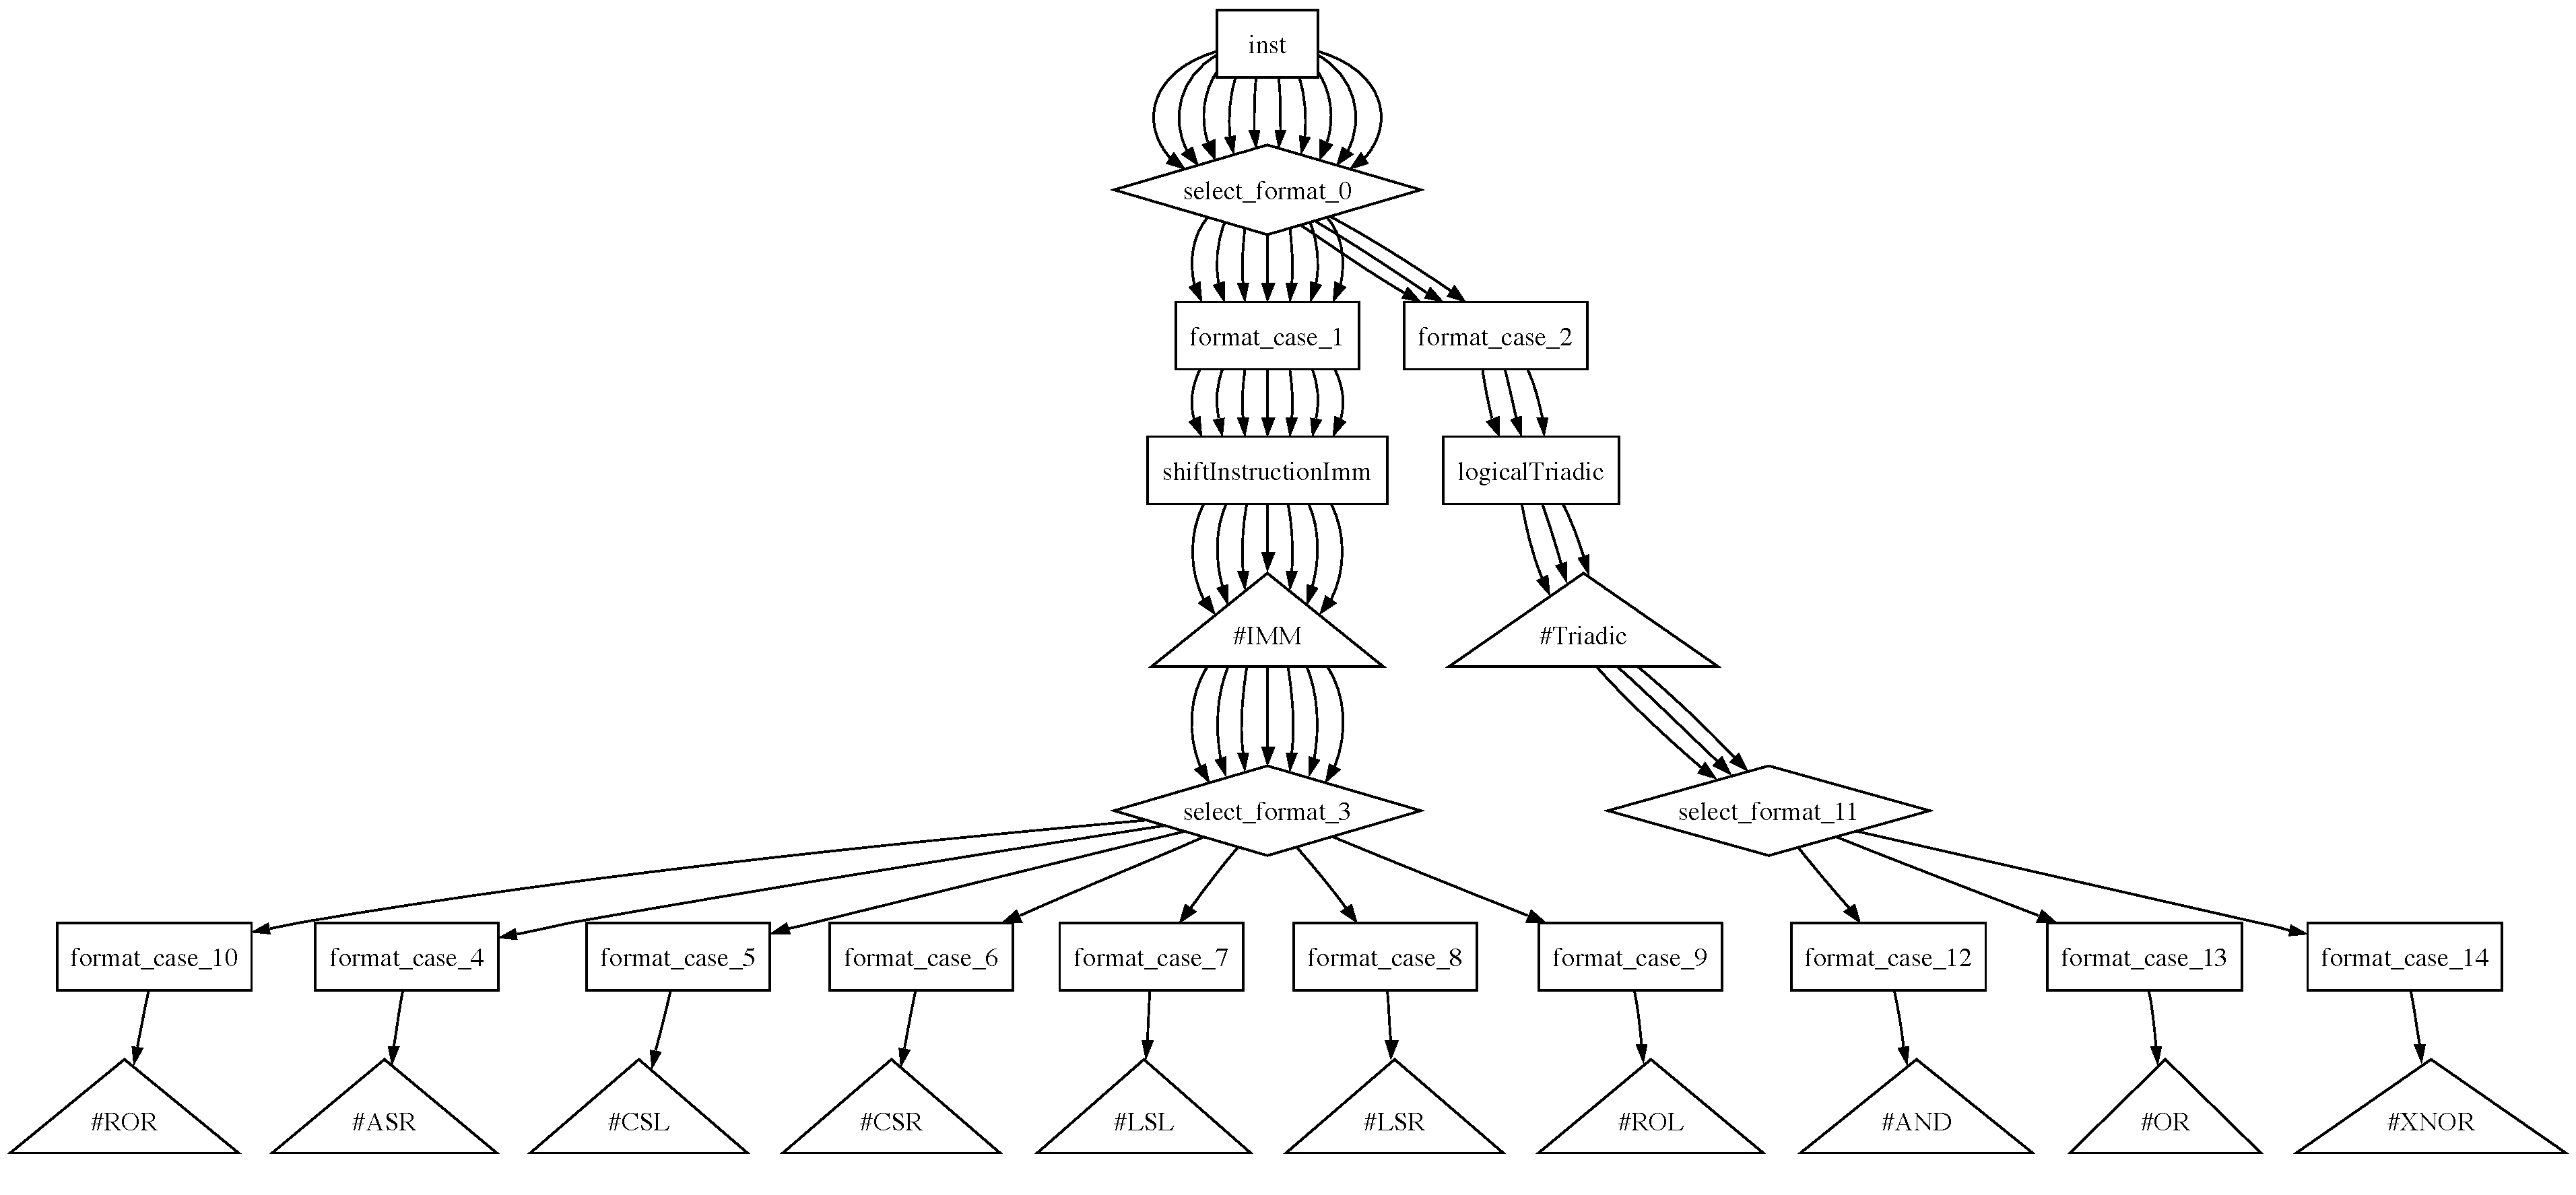
\includegraphics[width=\linewidth]{../common/images/format_all_test.pdf}
    \caption{Arbre généré à partir de la description du code binaire des instructions de décalage (shift) et les instruction triadiques (3 registres) sur la XGate.}
    \label{fig:formatAllTest}
  \end{center}
\end{figure}


This tree may become quickly difficult to display, that's why the second one only display \emph{tags} for each instruction, see figure \ref{fig:formatRefTest}. In this last figure, there are 2 distinct trees, because shift instruction and triadic instruction do not share anu common properties (no \emph{tags}).


\begin{figure}[h]		%% format Ref
  \begin{center}
    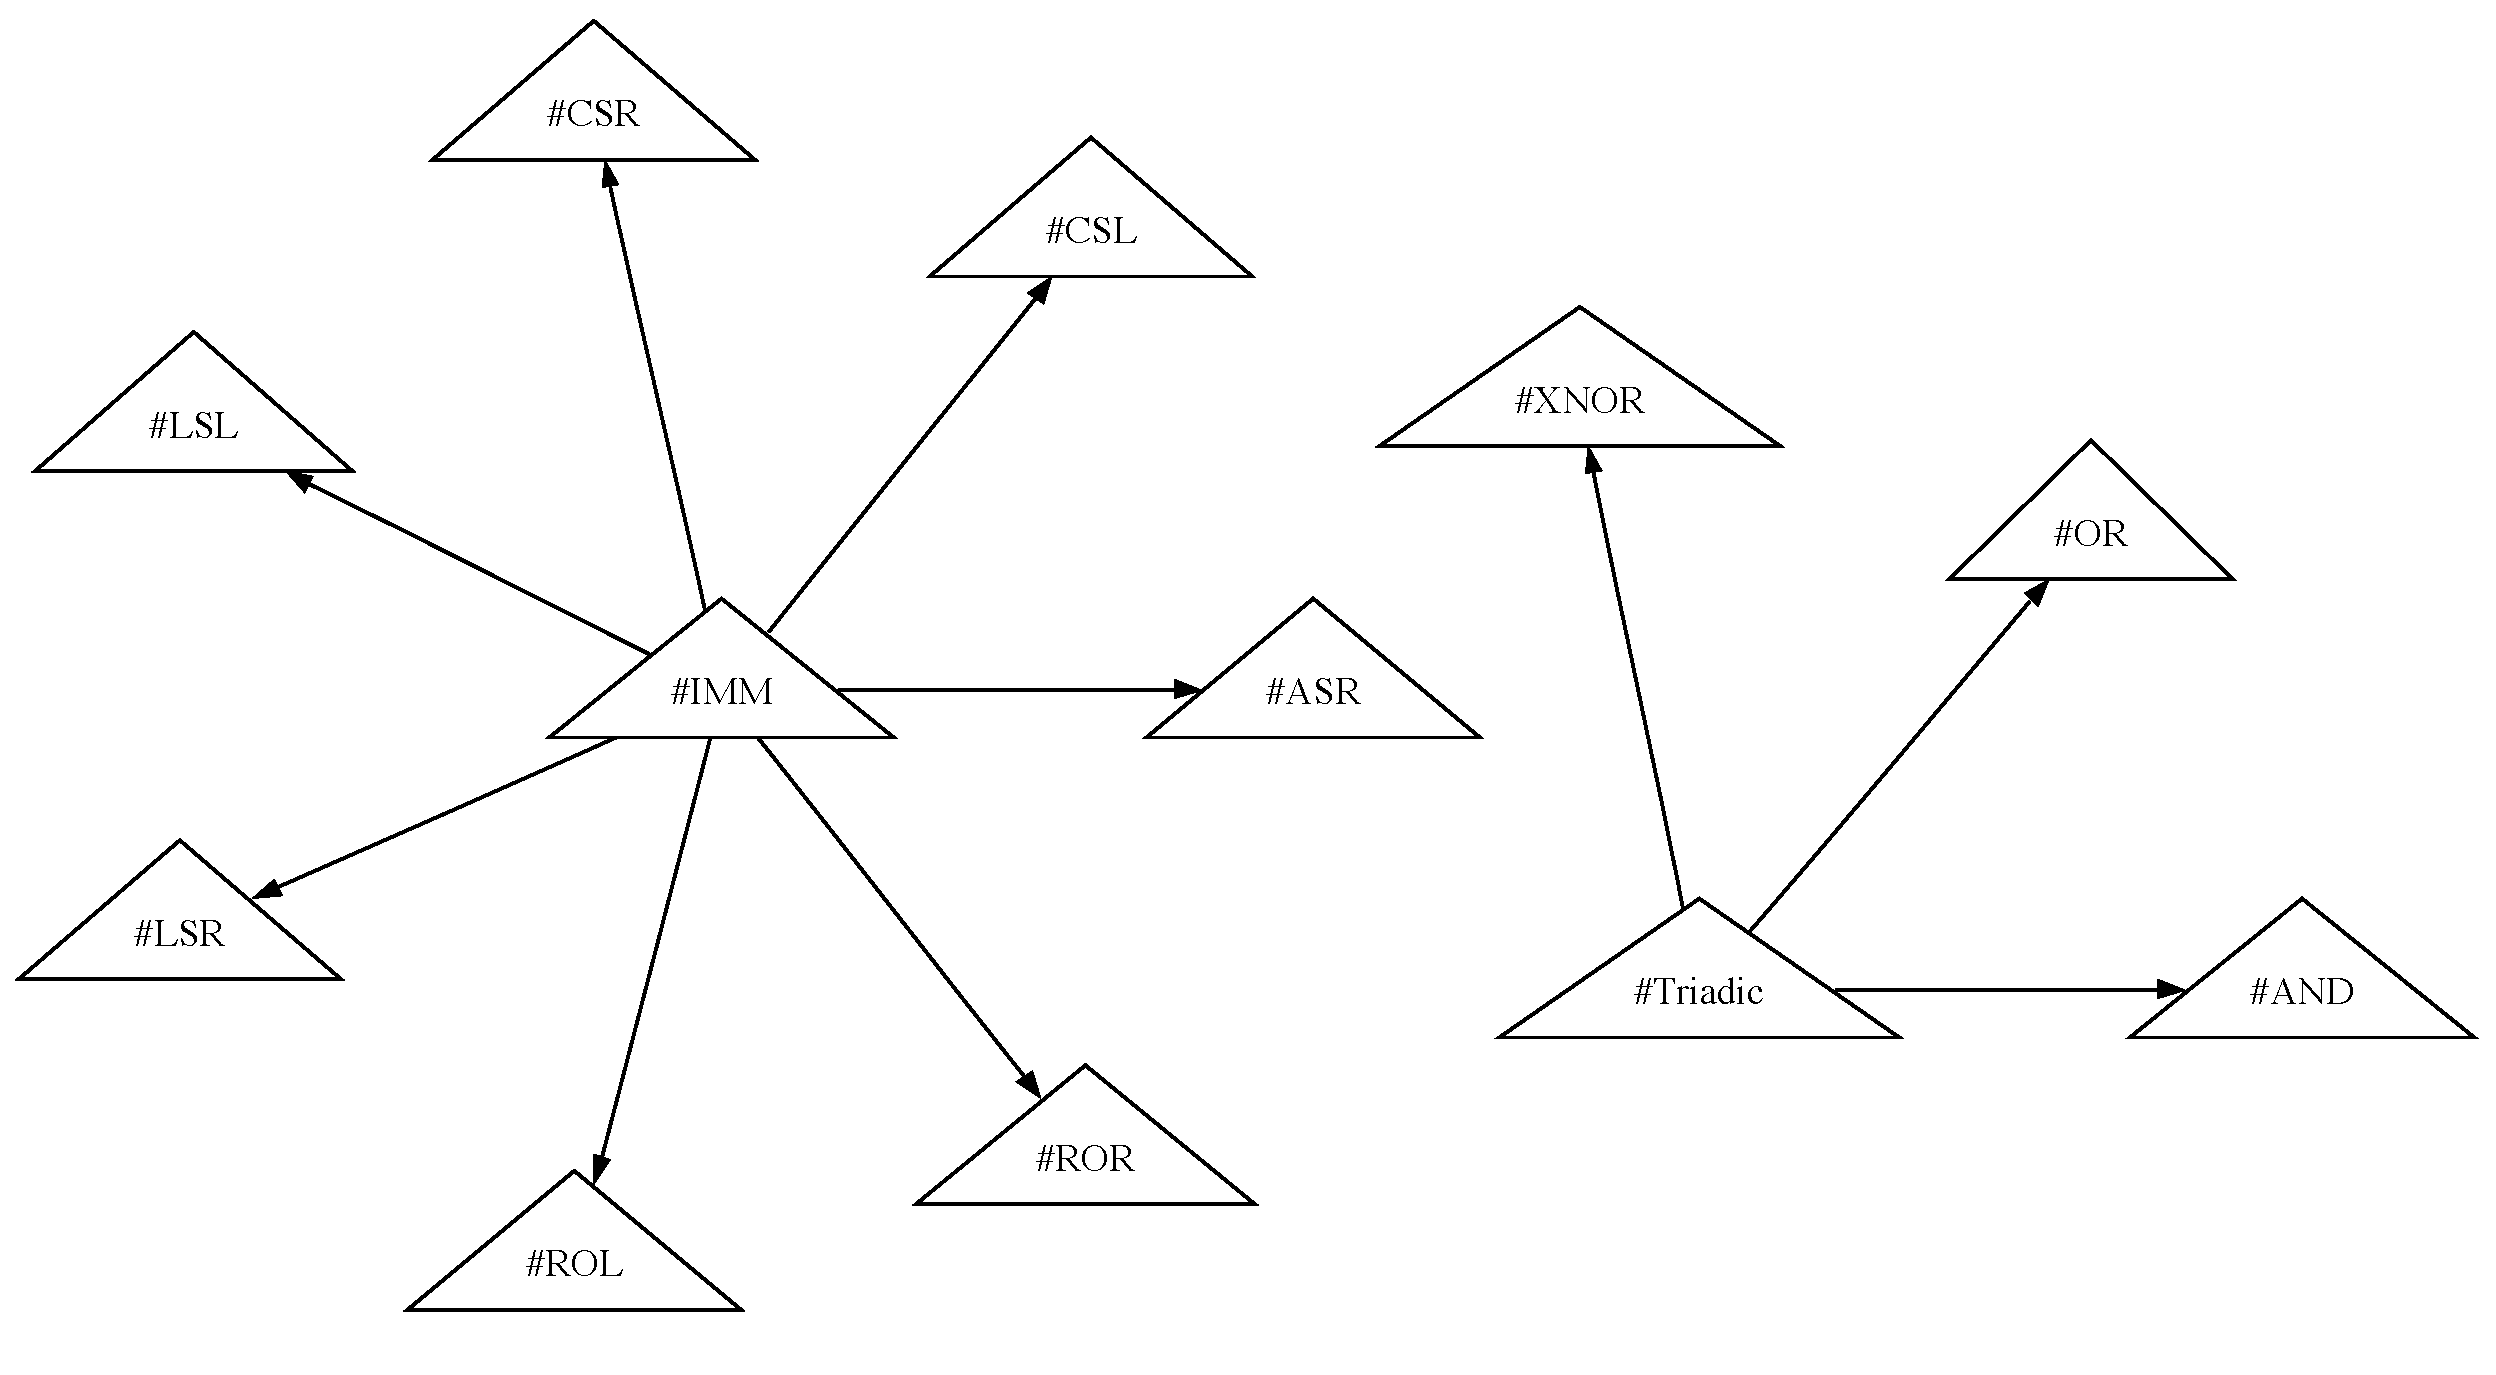
\includegraphics[width=\linewidth]{../common/images/format_ref_test.pdf}
    \caption{Trree generated from the description of shift and triadic instructions on the XGate instruction set. This tree is limited to tags.}
    \label{fig:formatRefTest}
  \end{center}
\end{figure}

Another file is \texttt{instruction.log} that embeds information about binary code of instructions:
\begin{itemize}
\item the path followed in the tree to get the instruction;
\item the \emph{instruction id}: Tags are ordered in alphabetical order;
\item the internal name used by instruction (debug in the generated \emph{C++} files)
\item the binary opcode (no date fields)
\item the name and size of data fields
\item the size of the instruction (word size is defined in section \emph{default});
\end{itemize}

For the triadic instruction \texttt{AND}, we get the following information:
\begin{verbatim}
inst 
-> select_format_0 
-> format_case_2 
-> logicalTriadic 
-> #Triadic 
-> select_format_11 
-> format_case_12 
-> #AND
	instruction id :#AND, #Triadic
	Internal name :test_AND_Triadic
	Binary coding :00010---------00
	data field(s) :rdIndex (3 bits)
	               rs1Index (3 bits)
	               rs2Index (3 bits)
	Instruction code size :1
\end{verbatim}

%TODO: debug -> fichier de log
%intérêt de l'archi avec les codes de l'ARM.
%indiquer que les performances du décodeur ne dépendent pas de la structure de l'arbre de description.

\section{variable size instruction set}
\label{sec:formatTailleVariable}
Variable size instruction set are described by adding binary words directly in the nodes.
In the following example, extracted from the \texttt{Freescale HCS12} instruction set (instruction word is 8 bits):
\begin{lstlisting}
format Instruction 
  select slice {7..0}
    case \x18 is inst_18 
    ....
  end select
end format

format inst_18 
  select slice +{7..0}
    case \m00010111 is #CBA       -- 17h
    ...
  end select
end format
\end{lstlisting}
In this example, the first node (\texttt{Instruction}) allows to defined the first word (as in fixed size instruction sets). Node \texttt{inst\_18} is called if this first word \texttt{0x18}. In format \texttt{inst\_18}, the \texttt{+} in the \texttt{select} part, line 9 implies that it is necessary to add a binary word to decode the instruction.
In this way, semantics of \texttt{+\{7..0\}} is: \emph{adding one word, and apply the \texttt{select} on the 8 bits of this new word.}

A \texttt{select} that have the following form:  \texttt{\{a..b\}\{c..d\}+\{e..f\}\{-\}\{g..h\}} show that 3 words are added for instructions de the current branch, and the \texttt{select} is applied on:
\begin{itemize}
\item bit field \texttt{a..b} of the previous word;
\item bit field \texttt{c..d} of the current word;
\item bit field\texttt{e..f} of the first word added;
\item the second added word is not used in the select structure;
\item bit field\texttt{g..h} of the third word added;
\end{itemize}
If there was no word previously added (there is only the current word), an error is generated.

If a new format is called in or after the \texttt{select}, le last added word becomes the current word.

This approach using relative access (adding words to previously added words) allow to describe easily instruction formats where the addressing mode is not always at the same place, as in the example figure \ref{fig:formatLongueurVariable}.

\begin{figure}		%% Small Example
  \begin{center}
    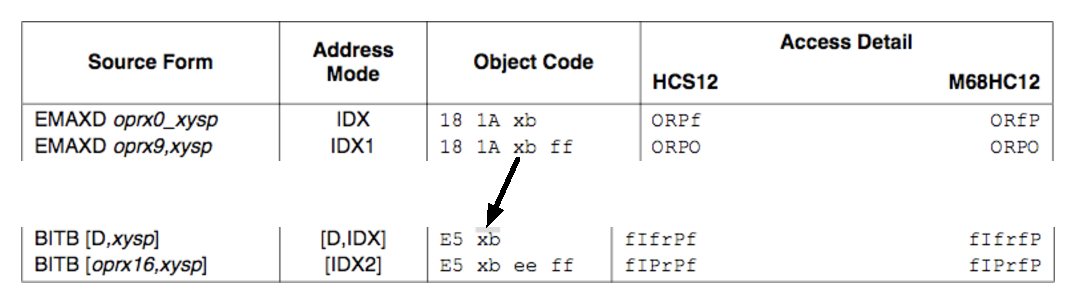
\includegraphics[width=0.8 \linewidth]{../common/images/formatLongueurVariable.pdf}
    \caption{Example of variable size instruction set, extracted form the documentation of HCS12. The addressing mode \texttt{xb} may be located at different places (source Freescale).}
    \label{fig:formatLongueurVariable}
  \end{center}
\end{figure}

%TODO: rajouter le fetch explicite!!!
%!TEX root = ./main.tex
%!TEX encoding = UTF-8 Unicode
\chapter[Description du comportement]{Description du comportement des instructions}
\label{chap:behavior}
\section{Introduction}

Dans ce chapitre, nous présentons comment le comportement des instructions est décrit. Plusieurs exemples, tirés des descriptions du HCS12 de Freescale et de son co-processeur XGate, illustrent la présentation. Le comportement des instructions est décrit de manière hiérarchique afin de mutualiser les comportements communs à plusieurs instructions.

La description du comportement des instructions s'appuie sur des objets appelés {\em component} dans le langage. Un component représente un dispositif matériel du processeur comme le banc de registres ou l'unité arithmétique et logique. Bien entendu, on peut décrire le comportement d'une instruction en se passant en partie des components (par exemple en utilisant l'opération d'addition du langage pour mettre en œuvre le comportement d'une instruction d'addition) mais cette façon de faire n'est pas recommandé. En effet, le comportement temporel d'une micro-architecture nécessite l'emploi de components car la concurrence d'accès est gérée en se basant sur les components.

\section{La vue comportementale dans \h}

La vue comportementale est formée par un ensemble de comportement. Un comportement peut faire appel à d'autres comportements plus élémentaires. Par exemple, un mode d'adressage peut constituer un comportement élémentaire qui sera employé par plusieurs comportement. Un comportement est rattaché à une instruction via sa signature. Contrairement à la vue format qui ne comprend qu'un seul arbre, la vue comportementale peut comprendre plusieurs arbres, chacun des arbres correspondant à des instructions ayant en commun un ou plusieurs comportements.

Un comportement est en définitive semblable à une fonction qui va faire appel à d'autres fonctions (sous comportement ou bien méthodes de components) pour effectuer les opérations nécessaires à l'exécution de l'instruction. Le listing suivant donne le canevas de déclaration d'un comportement:
\begin{lstlisting}
behavior <name>(<argumentsList>) [etiquette]
  <behaviorBody>
end behavior
\end{lstlisting}

Le {\tt <behaviorBody>} est formé d'élements de type:
\begin{itemize}
\item déclaration de variable (\ref{sec:behVar});
\item déclaration de {\em field} (\ref{sec:behField});
%\item \emph{étiquette};
\item appel à un autre nœud de type behavior (\ref{sec:behSubBeh});
\item structure de sélection, en utilisant le mot clé \texttt{select}. Voir section \ref{sec:behSelect};
\item \blocsdo\ permettant la mise en œuvre d'algorithmes. Voir section \ref{sec:behDo}.
\end{itemize}

\subsection{Arguments d'un comportement}

Un comportement, à la condition qu'il ne s'agisse pas d'un comportement racine), peut prendre 1 ou plusieurs arguments en entrée ou en sortie. Un argument est typé. Un argument en sortie est signalé par le mot clé {\tt out}. L'utilisation est la même que le passage d'arguments à une fonction.
\begin{lstlisting}
behavior shiftInstructionBehavior(out u16 rdValue, u16 source)\end{lstlisting}
Ici, 2 aurguments sont spécifiés. Le premier, {\tt rdValue}, est un argument de sortie (c'est à dire qu'il sera valué par {\tt shiftInstructionBehavior} et que la valeur sera disponible pour le comportement qui appelle {\tt shiftInstructionBehavior}). Le second, {\tt source} est un argument en entrée.

\subsection{Déclaration de variables}
\label{sec:behVar}

Il est possible de déclarer des variables locales dans un comportement selon \ref{sec:TypeDonnees}. Les variables ne peuvent être déclarées à l'intérieur d'un \blocdo.

\subsection{Référencement d'un champ}
\label{sec:behField}

Les champs de l'instruction contenant des constantes numériques peuvent être décla\-rés dans un comportement afin de les référencer et d'employer leur valeur dans un calcul. Le mot clé {\em field} permet de déclarer un champ:
\begin{lstlisting}
  field u3 regIndex;
\end{lstlisting}
Ici, {\tt regIndex} est un champ qui a été extrait de l'instruction dans un format (voir la section \ref{sec:operandeFormat}). \h\ vérifie la cohérence de type (taille et signe) et signale une erreur en cas d'incohérence. Un {\em field} est bien entendu une constante.

\subsection{Appel à un autre comportement}
\label{sec:behSubBeh}

Un appel à une autre comportement est effectué en indiquant le nom du comportement et les arguments nécessaire. Un appel à un comportement ne peut être effectué à l'intérieur d'un \blocdo :
\begin{lstlisting}
behavior shiftInstructionType(out u16 source)
  ...
end behavior

behavior shiftInstructionBehavior(out u16 rdValue, u16 source)
  ...
end behavior

behavior shiftInstruction() #SHIFT
  ...
  u16 rdValue;
  u16 source;
  shiftInstructionType(source)
  shiftInstructionBehavior(rdValue, source)
  ...
end behavior
\end{lstlisting}
Ici, dans le comportement {\tt shiftInstruction}, deux variables locales, {\tt rdValue} et {\tt source} sont déclarées puis deux comportements, {\tt shiftInstructionType} et {\tt shiftInstruction\-Behavior}, sont appelés. {\tt shiftInstructionType} value source qui est ensuite passé en argument à {\tt shiftInstructionBehavior} qui value {\tt rdValue}.

\subsection{Structure de sélection}
\label{sec:behSelect}

L'instruction {\tt select} permet de choisir entre plusieurs comportement en fonction d'une étiquette ou d'un comportement appelé (également étiqueté):
\begin{lstlisting}
  select
    case #ROL do rdValue := ALU.ROL(rdValue, source); end do
    case #ROR do rdValue := ALU.ROR(rdValue, source); end do
  end select
\end{lstlisting}
Ici, selon qu'il s'agit de l'étiquette \#ROL ou \#ROR, l'un ou l'autre des \blocsdo\ est pris en compte.

\begin{lstlisting}
  select
    case logicImmAndArithImmUpdateNoReg(rdValue, imm8)
    case logicImmAndArithImmUpdateReg(rdValue, imm8, rdIndex)
  end select;
\end{lstlisting}
Ici, l'un ou l'autres des comportements est pris en compte. Les deux types de {\tt case} peuvent bien entendu êtres présents dans le même {\tt select}.

Un {\tt select} ne peut pas apparaître dans un \blocdo.

\subsection{Les \blocsdo}
\label{sec:behDo}

Les \blocsdo\ permettent de donner l'algorithme de l'instruction. Ils peuvent contenir des accès aux composants via leurs méthodes, des structures de contrôle {\em if ... then ... else} et des expressions telles que décrites dans la section \ref{sec:expressions}. Le comportement suivant, issu de la description du XGate, est un exemple de \blocdo. 
\begin{lstlisting}
behavior loadStoreType(u1 accessType, u16 addr, u3 regIndex)
  select
    case #LOAD
      do
         if accessType = 0 then
           u8 val := mem.read8(addr);
           GPR.write8(regIndex, val);
         else
           u16 val := mem.read16(addr);
           GPR.write16(regIndex, val);
         end if;
      end do
    case #STORE 
      do
         if accessType = 0 then
           u8 val := GPR.read8(regIndex);
           mem.write8(addr, val);
         else
           u16 val := GPR.read16(regIndex);
           mem.write16(addr, val);
         end if;
      end do
  end select
end behavior
\end{lstlisting}
Ici, selon qu'il s'agit d'une instruction de chargement (\#LOAD) ou de rangement (\#STO\-RE), l'un ou l'autre des comportement est sélectionné. {\tt accessType} spécifie la taille de la donnée à accéder en mémoire. Les méthodes ad-hoc des composants {\tt GPR} (registres généraux) et {\tt mem} sont appelées en conséquence.

\section{Les composants matériels}
\label{sec:component}
Un composant matériel représente une partie matérielle (ALU, bloc mémoire, \ldots), sa description est encapsulée et contient:
\begin{itemize}
\item des variables membres;
\item des méthodes associées.
\end{itemize}
Soit par exemple un composant \texttt{Fetcher} chargé de la gestion du compteur programme:
\begin{lstlisting}
component Fetcher {
  program counter u16 pc; -- generate get and set methods.

  void reset() {
    pc := 0;
  }

  void branch(s16 offset) {
    pc := (u16)((s16)(pc) + offset);
  }
}
\end{lstlisting}
Ce composant utilise une variable membre, qui est un registre (ici un registre spécifique: le compteur programme). Il y a aussi 2 méthodes qui sont associées \texttt{reset} et \texttt{branch}, dont la syntaxe ressemble beaucoup à celle du C. Au niveau d'un \emph{behavior}, on peut appeler les différentes méthodes d'un composant, à l'intérieur d'un bloc \texttt{do .. end do} de la manière suivante: \texttt{<componentName>.<methodName>}, soit ici par exemple: \texttt{Fetcher.branch(10)}. 

Cette approche ressemble beaucoup à une approche objet, cependant, il n'y a pas de notion d'instance associée à un composant.
\subsection{définition d'une méthode}
Une méthode, comme introduit précédemment, est défini de la manière suivante:
\begin{verbatim}
<typeRetour> nomMethod(<paramètres>)
{
  <implémentation>
}
\end{verbatim}
où:
\begin{itemize}
\item \texttt{<typeRetour>} est le type de retour de la fonction (\texttt{u8}, \texttt{s5}, ... ou \texttt{void});
\item \texttt{<paramètres>} correspond aux différents paramètres (comme en C). Les paramètres sont des entrées uniquement par défaut. un paramètre peut être déclaré en sortie s'il est précédé du mot clé \texttt{out}: \texttt{u8 param1, u16 param2, out u32 paramOut};
\item \texttt{<implémentation>} est la même chose que dans la section \ref{sec:behDo}.
\end{itemize}

\subsection{Variables membres}
Les variables membres ne sont accessible que dans les méthodes du même composant (encapsulation). Cependant, les registres (voir section \ref{sec:defReg}) ont une portée plus large et peuvent être utilisé dans n'importe quelle autre endroit de la description.

\subsection{Utilisation des composants}
Les composants sont utilisés pour faire le lien entre la partie comportementale (\emph{behavior}) et la description de la micro-architecture. Cette description, permettant de décrire le pipeline n'est actuellement pas finalisée.
Ainsi, dans la description d'une instruction, certaines partie du comportement peuvent être décrite soit dans un \texttt{behavior}, soit dans un \texttt{component}. Par exemple, au lieu d'appeler \texttt{Fetcher.branch(..)}, il est tout à fait possible de modifier directement la valeur de \texttt{PC} dans un \texttt{behavior}. Cependant, l'information sur l'utilisation des composant va servir dans un deuxième temps, soit dans la description de la micro-architecture, soit dans la vue \texttt{timing} (voir chapitre \ref{chap:timing}).

Dans la description de la micro-architecure, il est notamment possible d'associer l'utilisation d'une méthode d'un composant à un étage du pipeline. Ainsi, il est possible de \emph{mapper} le comportement de l'instruction directement sur le pipeline.

A contrario, si l'accès est fait dans le \texttt{behavior}, tout \emph{mapping} est impossible. Cette approche est aussi utile pour les comportement qui n'affectent pas temporellement l'exécution. Considérons par exemple une instruction post-incrémentée, dont l'incrémentation est réalisée par un matériel dédié. Dans ce cas, il est inutile de mapper cette post-incrémentation sur le pipeline, car elle n'affecte en rien les temps d'exécution.

\subsection{Initialisation}
\label{sec:initComponent}
L'initialisation d'un composant est réalisé implicitement si un composant possède une méthode \texttt{reset} qui ne prend aucun argument:
\begin{lstlisting}
  void reset() {
    pc := 0;
  }
}
\end{lstlisting}
Ceci permet notamment d'initialiser les variables d'un composant, ainsi que les registres défini dans le composant.

%\section{Exemple de mise en œuvre}


%!TEX root = ./main.tex
%!TEX encoding = UTF-8 Unicode
\chapter{Description of instructions syntax code}
\label{chap:syntax}
\section{Introduction}
In this chapter, we will present how to describe the instruction set syntax for a given processor. To illustrate, we will use different examples extracted from the description of the AVR micro-controller, the Freescale HCS12 processor and its co-processor XGate. 

The syntax view follows the same principle as the other two views (format and behavior). It describes the textual format of instructions by concatenating strings. In other words, it assigns a textual syntax for each instruction signature to allow, for example, the disassembling.

\section {Arborescent structure of the syntax view in \harmless}
As in the other two views (format and behavior), the syntax view consists of a set of trees, where a node describes a part of the syntax of one or more instructions. Each branch of the tree represents an instruction.

In this view, each node is written using the following syntax:

\begin{lstlisting}
syntax <name> [tag]
  <syntaxBody>
end syntax
\end{lstlisting}

A syntax node can call another node, or make a selection structure between different nodes, using the \texttt{select} structure type. This approach is common to the 4 views (\texttt{format}, \texttt{syntax}, \texttt{behavior} and \texttt{timing}) and is described in more details in section \ref{sec:modelisationArborescente}.

%Nous allons ici nous intéresser plus particulièrement au corps d'un nœud \texttt{<syntaxBody>} qui est spécifique à la génération d'un mnémonique, tout en donnant quelques exemples liés à la structure arborescente de la description des éléments de type \texttt{syntax}.
%
%\section{La partie \texttt{<syntaxBody>}}
%
%La partie \texttt{<syntaxBody>} est une succession d'éléments de type (\ref{sec:syntaxBody}):
%\begin{itemize}
%\item \emph{étiquette};
%\item étiquette (l'ensemble des étiquettes définissant la signature de l'instruction), voir \ref{sec:syntaxEtiquette};
%\item appel à un autre nœud de type \texttt{syntax}, en utilisant le nom de l'élément \texttt{syntax} appelé;
%\item structure de sélection, en utilisant le mot clé \texttt{select}, voir section \ref{sec:syntaxSelect};
%\item déclaration de \emph{field}, voir section \ref{sec:syntaxField};
%\item chaîne de caractères suivie ou non d'un ou plusieurs variables déclarées. Cette chaîne constitue le mnémonique à proprement parler de l'instruction, voir section \ref{sec:syntaxChaineCaract};
%\item structure de sélection permettant de mettre en œuvre un choix dynamiquement (en fonction de la valuer des données), voir section \ref{sec:syntaxIf}.
%\end{itemize}
%
%\subsection{Les étiquettes}
%\label{sec:syntaxEtiquette}
%Comme dans la vue binaire, les nœuds sont associés à des étiquettes (tags) dont l'ensemble forme la signature de l'instruction. Lors de l'évaluation des différents chemins des instructions, les étiquettes sont récoltées pour former la signature de l'instruction. On s'intéresse à un \emph{ensemble}, donc le nombre d'étiquettes de même nom n'est compté qu'une fois, et il n'y a pas de relation d'ordre, voir \ref{sec:signature}.
%
%\subsection{Structure de sélection \texttt{select}}
%\label{sec:syntaxSelect}
%Le mot clé {\tt "select"} permet de créer différentes branches dans l'arborescence, comme indiqué dans \ref{sec:modelisationArborescente}.
%
%La syntaxe générale de cette structure est la suivante:
%\begin{lstlisting}
%syntax test
%  <syntaxBody1>
%  select 
%    case <syntaxBody2>
%    case <syntaxBody3>
%    ...
%  end select;
%  <syntaxBody4>
%end syntax
%\end{lstlisting}
%Ainsi, dans cette architecture, 2 instructions sont définies. Elles sont composées respectivement des éléments:
%\begin{itemize}
%\item \texttt{<syntaxBody1>}, \texttt{<syntaxBody2>} et \texttt{<syntaxBody4>};
%\item \texttt{<syntaxBody1>}, \texttt{<syntaxBody3>} et \texttt{<syntaxBody4>};
%\end{itemize}
% Ainsi, la structure \texttt{select} permet de mutualiser les parties communes aux mnémoniques de différentes instructions (\texttt{<syntaxBody1>} et \texttt{<syntaxBody4>}), et de les différencier sur d'autres parties.
%
%Bien entendu, les étiquettes dans les parties \texttt{<syntaxBody2>} et  \texttt{<syntaxBody3>} doivent être différentes pour différencier les différents chemins (et constituer les signatures des instructions).
%
%Soit par exemple (issu du jeu d'instructions de l'AVR):
%\begin{lstlisting}
%syntax classicImm8 
%  field u4 regIndex -- should add 16 to the result
%  field u8 k
%  select
%    case #ANDI "ANDI" -- or CBR with ~k 
%    case #CPI  "CPI"
%    case #ORI  "ORI"
%    case #SBCI "SBCI"
%    case #SUBI "SUBI"
%  end select
%  " R\d, \x", regIndex+16, k
%end syntax
%\end{lstlisting}
%Cet exemple permet de construire la syntaxe de 5 instructions différentes, en mutualisant la récupération des champs issus du \texttt{format}, ainsi que leur affichage. Dans ce cas, les signatures des instructions ne comprennent qu'une seule étiquette.
%
%Cette structure en \texttt{select} est résolue de manière statique à la génération du simulateur. Par conséquent, 5 instructions seront générées, avec chacune leur code associé. Aucun impact sur les performances n'est associé à la multiplication des éléments \texttt{select}.
%
%\subsection{Récupération des champs du format binaire}
% \label{sec:syntaxField}
% Dans la vue syntaxique, il est nécessaire de pouvoir récupérer la valeur des différents champs extrait du code binaire de l'instruction. L'opération d'extraction de ces champs dans la partie binaire de l'instruction est réalisé dans la partie \texttt{format} de la description. Dans la partie \texttt{syntax}, on se contente de récupérer ces différents champs sous la forme de constantes.
% 
% Ainsi, le mot clé {\tt "field"} permet de référencer un champ qui est extrait de l'instruction dans la vue binaire.\harmless\ étant un langage fortement typé, le type des différents champs doit correspondre exactement avec celui extrait de la vue binaire:
%
%\begin{lstlisting}
%field <typeDonnee> <nom_du_champ>
%\end{lstlisting}
%
%Où {\tt <typeDonnee>} est un type de donnée, comme défini dans la section \ref{sec:TypeDonnees} (\texttt{u3} pour un entier non signé sur 3 bits, \texttt{s5} pour un entier signé sur 5 bits, \ldots). Il doit correspondre au nombre de bits extraits dans la vue binaire pour la même variable (ou être plus grande).
%
%Par exemple, une donnée non signée nommée {\tt "rs1Index"} est déclarée dans la vue binaire de la façon suivante:
%
%\begin{lstlisting}
%rs1Index := slice{7..5}
%\end{lstlisting}
%
%Dans la vue syntaxique, sa valeur sera importée sous la forme:
%
%\begin{lstlisting}
%field u3 rs1Index
%\end{lstlisting}
%
%Ici, nous pouvons remarquer que la taille du champ est égale à 3, ce qui correspond bien au 3 bits extraits (bit 7, 6 et 5).
%
%\subsection{Les  chaînes de caractères}
%\label{sec:syntaxChaineCaract}
%Dans la vue syntaxique, une chaîne de caractères est une suite de caractères entre guillemets. 
%
%Lors de l'évaluation d'une branche de la description (qui modélise une instruction), les différentes chaînes de caractères sont concaténées pour former la mnémonique de l'instruction.
%
%Avec une approche similaire à celle de la fonction \texttt{printf} du langage \texttt{C}, il est possible de faire référence à des données qui sont définies en dehors de la chaîne de caractères, en utilisant des séquences d'échappement. Chaque séquence d'échappement est alors remplacée par une expression:
%
%\begin{lstlisting}
%<chaine_de_caracteres>, <expression_0>, ..., <expression_n>
%\end{lstlisting}
%
%soir par exemple:
%\begin{lstlisting}
%    "CLR R\d", rdIndex
%    ...
%    "LDI R\d, \x", regIndex+16, k
%\end{lstlisting}
%Il est indispensable d'avoir le même nombre de caractères d'échappements que d'expressions.
%
%\subsubsection{Séquences d'échappement dans les chaînes de caractères}
%Les séquences d'échappement permettent de faire référence aux expressions qui suivent la chaîne de caractère. Les 4 séquences d'échappement permettent de définir la base utilisée pour l'affichage:
%\begin{table}[!h]
%\begin{center}
%\begin{tabularx}{0.7 \columnwidth}{|X|c|}
%\hline
%\bf séquence d'échappement & \bf Signification \\  \hline
%\textbackslash b & Base binaire \\ \hline
%\textbackslash d & Base décimal \\ \hline
%\textbackslash x & Base hexadécimal \\ \hline
%\textbackslash o & Base octal \\ \hline
%\end{tabularx}
%\caption{Base utilisée pour les différentes séquences d'échappement}
%\label{tab:type-donnee}
%\end{center}
%\end{table}
%
%De plus, pour chaque base, \harmless\ donne la possibilité de préciser les caractères avant (\texttt{prefix}) et après (\texttt{suffix}) l'expression de manière globale, selon la syntaxe suivante: 
%
%\begin{lstlisting}
%number syntax <base> <prefix_ou_suffix> <chaine_de_caracteres>
%\end{lstlisting}
%
%Où {\tt <base>} peut être {\tt binary, octal, hexadecimal} ou {\tt decimal}. {\tt <prefix\_ou\_suffix>} peut être {\tt prefix} ou {\tt suffix}, et \texttt{<chaine\_de\_caracteres>} est une suite quelconque de caractères entres guillemets. Ces directives sont généralement placées au début de la section où sont placés les éléments \texttt{syntax}.
%Voici un exemple: 
%
%\begin{lstlisting}
%number syntax octal prefix "o"
%number syntax hexadecimal prefix "0x"
%number syntax hexadecimal suffix "h"
%\end{lstlisting}
%
%Ainsi, à travers cet exemple, la description suivante:
%\begin{lstlisting}
%    "LDI R\d, \x", regIndex+16, k
%\end{lstlisting}
%conduira à l'affichage suivant (si k=5, et regIndex = 3):
%\begin{verbatim}
%    "LDI R19, 0x5h"
%\end{verbatim}
%
%\subsection{La structure \texttt{if ... then ... else}}
%\label{sec:syntaxIf}
%La structure conditionnelle \texttt{if ... then ... else} permet de faire un choix dynamique en fonction des différents champs d'une instruction. Elle est utilisée de la manière suivante:
%\begin{lstlisting}
%if <condition> then
%  <ifSyntaxStatement>
%[elseif <condition> then
%  <ifSyntaxStatement>
%]
%[else 
%  <ifSyntaxStatement>
%]
%end if;
%\end{lstlisting}
%
%La \texttt{<condition>} est une expression booléenne classique (voir \ref{sec:expressions}).
%La partie \texttt{<ifSyntaxStatement>} n'est prise en compte que si la condition est vraie. On peut avoir:
%\begin{itemize}
%\item une chaîne de caractères;
%\item une autre condition (\texttt{if..then..end if}.
%\end{itemize}
%
%Par contre, comme la condition est évaluée dynamiquement (à l'exécution), il n'est pas possible de faire intervenir des informations qui sont utilisées statiquement (au moment de la génération des sources du simulateur), comme par exemple une étiquette ou une structure de type \texttt{select}.
%
%Les parties {\tt "elseif"} et {\tt "else"} sont facultatives.
%
%Cette approche permet notamment de définir les \emph{mnémoniques simplifiées} associées à certaines instructions. Dans l'exemple suivant, une instruction de type \texttt{OR Rd, Ra, Ra} est simplifiée en \texttt{MOV Rd, Ra}:
%\begin{lstlisting}
%syntax orOperation #TriadicInst #OR
%  field u3 rs1Index
%  field u3 rs2Index
%  field u3 rdIndex
%  if rs1Index = rs2Index then
%    "MOV R\d, R\d", rdIndex, rs1Index
%  else
%    "OR R\d, R\d, R\d", rdIndex, rs1Index, rs2Index
%  end if;
%end syntax
%\end{lstlisting}
%
%\section{Assemblage du tout}
%
%Prenons comme exemple l'ensemble d'instructions faisant intervenir 3 registres dans la XGate. Dans la documentation technique, cet ensemble d'instructions est résumé par le tableau \ref{tab:triadic}.
%
%\begin{table}[!h]
%\begin{center}
%\begin{tabularx}{1.1 \columnwidth}{|c|c|c|c|c|c|c|c|c|c|c|c|c|c|c|c|X|} 
%\hline
%\bf Functionality & \bf 15 & \bf 14 & \bf 13 & \bf 12 & \bf 11 & \bf 10 & \bf 9 & \bf 8 & \bf 7 & \bf 6 & \bf 5 & \bf 4 & \bf 3 & \bf 2 & \bf 1 & \bf 0\\  \hline
%\bf Logical triadic & \multicolumn{16}{c|}{ } \\ \hline
%AND RD, RS1, RS2 & 0 & 0 & 0 & 1 & 0 & \multicolumn{3}{c|}{RD} & \multicolumn{3}{c|}{RS1} & \multicolumn{3}{c|}{RS2} & 0 & 0 \\ \hline
%OR RD, RS1, RS2 & 0 & 0 & 0 & 1 & 0 & \multicolumn{3}{c|}{RD} &  \multicolumn{3}{c|}{RS1} & \multicolumn{3}{c|}{RS2} & 1 & 0 \\ \hline
%XNOR RD, RS1, RS2 & 0 & 0 & 0 & 1 & 0 & \multicolumn{3}{c|}{RD} & \multicolumn{3}{c|}{RS1} & \multicolumn{3}{c|}{RS2} & 1 & 1 \\ \hline
%\bf Arithmetic triadic & \multicolumn{16}{c|}{For compare use SUB R0,Rs1,Rs2} \\ \hline
%SUB RD, RS1, RS2 & 0 & 0 & 0 & 1 & 1 & \multicolumn{3}{c|}{RD} & \multicolumn{3}{c|}{RS1} & \multicolumn{3}{c|}{RS2} & 0 & 0 \\ \hline
%SBC RD, RS1, RS2 & 0 & 0 & 0 & 1 & 1 & \multicolumn{3}{c|}{RD} & \multicolumn{3}{c|}{RS1} & \multicolumn{3}{c|}{RS2} & 0 & 1 \\ \hline
%ADD RD, RS1, RS2 & 0 & 0 & 0 & 1 & 1 & \multicolumn{3}{c|}{RD} & \multicolumn{3}{c|}{RS1} & \multicolumn{3}{c|}{RS2} & 1 & 0 \\ \hline
%ADC RD, RS1, RS2 & 0 & 0 & 0 & 1 & 1 & \multicolumn{3}{c|}{RD} & \multicolumn{3}{c|}{RS1} & \multicolumn{3}{c|}{RS2} & 1 & 1 \\ \hline
%\end{tabularx}
%\caption{Ce tableau représente l'ensemble d'instructions  {\tt "triadic"}, comme trouvé dans le datasheet de la XGate.}
%\label{tab:triadic}
%\end{center}
%\end{table}
%
%Dans  \harmless\ , cet ensemble d'instructions peut être décrit comme suit:
% 
%\begin{lstlisting}
%syntax triadicInstruction #TriadicInst 
%  field u3 rs1Index
%  field u3 rs2Index
%  field u3 rdIndex
%  triadicOperation
%  " R\d, R\d, R\d", rdIndex, rs1Index, rs2Index
%end syntax
%
%syntax triadicOperation 
%  select
%    case #AND  "AND"
%    case #XNOR "XNOR"
%    case #SBC  "SBC"
%    case #ADD  "ADD"
%    case #ADC  "ADC"
%  end select
%end syntax
%
%syntax orOperation #TriadicInst #OR
%  field u3 rs1Index
%  field u3 rs2Index
%  field u3 rdIndex
%  if rs1Index = rs2Index then
%    "MOV R\d, R\d", rdIndex, rs1Index
%  else
%    "OR R\d, R\d, R\d", rdIndex, rs1Index, rs2Index
%  end if;
%end syntax
%
%syntax subOperation #TriadicInst #SUB
%  field u3 rs1Index
%  field u3 rs2Index
%  field u3 rdIndex
%  if rdIndex = 0 then
%    "CMP R\d, R\d",rs1Index, rs2Index
%  else
%    "SUB R\d, R\d, R\d", rdIndex, rs1Index, rs2Index
%  end if;
%end syntax
%
%\end{lstlisting}
%
%La vue syntaxique a une structure arborescente, dont la représentation graphique est donnée dans le schéma \ref{fig:TriadicInst}. On peut noter que les 2 premiers éléments \texttt{syntax} permettent de traiter les cas généraux, et que les 2 suivants permettent de traiter des cas particuliers (car contenant des mnémoniques simplifiées).
%
%\begin{figure}		
%  \begin{center}
%    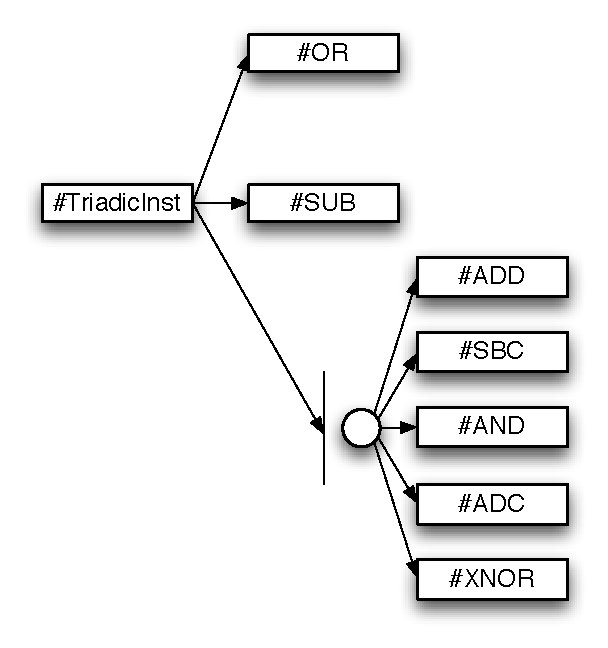
\includegraphics[width=0.5 \linewidth]{../common/images/TriadicInst.pdf}
%    \caption{Syntaxe de l'ensemble d'instructions triadic.}
%    \label{fig:TriadicInst}
%  \end{center}
%\end{figure}

%%!TEX root = ./main.tex
%!TEX encoding = UTF-8 Unicode
\chapter{Description fonctionnelle des éléments de mémorisation.}
\label{sec:mem_program}

La description des éléments de mémorisation est nécessaire pour la génération d'un simulateur de jeu d'instruction, mais aussi d'un simulateur précis au cycle. Dans cette dernière approche, il sera de plus nécessaire de rajouter des informations relatives au comportement temporel de la mémoire.

Dans cette version, la hiérarchie mémoire n'est pas modélisée (système de cache). En effet, son comportement est normalement transparent d'un point de vue fonctionnel, bien qu'il y ait la possibilité de gérer quelquefois les caches (cache locking, scratch pad, \ldots).

\section{Généralités}
\subsection{Organisation}
La mémoire est définie à l'intérieur d'un composant (voir section \ref{sec:component}). Ceci présente un double avantage:
\begin{itemize}
\item il est possible de rajouter des méthodes dans le composant, afin de simplifier l'accès à la mémoire (rajout de méthodes \texttt{push/pop} pour modéliser une pile, modélisation de mémoire paginée, \ldots
\item il est aussi possible de permettre l'accès à plusieurs zones de mémoire de manière transparente. Par exemple, une zone de mémoire RAM (largeur 16 bits) et une EEPROM (largeur 8 bits) dans le même espace d'adressage.
\end{itemize}

Une zone de mémoire est déclarée en utilisant le mot clé \texttt{memory}. Certains paramètres permettent de définir la zone mémoire. 

\subsubsection{Plage d'adresse}
La plage d'adresse est définie de la manière suivante: \texttt{address := startAddr..endAddr}, où \texttt{startAddr} et \texttt{endAddr} sont des valeurs numériques. La zone de mémoire est alors définie sur la zone d'adresse qui commence à \texttt{startAddr} \emph{inclus}, et va jusqu'à \texttt{endAddr} \emph{exclus}. Il est à noter qu'il est possible d'utiliser les suffixes \texttt{kb} et \texttt{mb} au valeurs numériques (voir section
\ref{sec:nombres}):
\begin{lstlisting}
    address := 0..128kb  
\end{lstlisting}

\subsubsection{Largeur du bus mémoire}
La largeur d'accès est définie par le mot clé \texttt{width}. Elle permet de définir la largeur maximale d'un accès en mémoire. L'accès reste possible pour les puissances de 2 inférieures. Par exemple:
\begin{lstlisting}
    width := 20  
\end{lstlisting}
L'accès sera possible sur 20 bits, mais aussi sur 16 bits et 8 bits.

\subsubsection{Type de mémoire}
Le type de mémoire est actuellement \texttt{RAM}, \texttt{ROM}, ou \texttt{register}. Dans le cas de la ROM, il n'est pas possible de faire des accès en écriture, mais il reste possible de mettre le code programme au démarrage, voir la section \ref{sec:memProgramme}. Exemple:
\begin{lstlisting}
    type := RAM
\end{lstlisting}

Il n'y a actuellement pas de différence entre les types \texttt{RAM} et \texttt{register}.

\subsubsection{Décalage}
Il est possible de faire un décalage des adresses pour une utilisation simplifiée, à l'aide du mot clé \texttt{stride}. Soit par exemple une zone de 16 registres généraux sur un processeur 16 bits. Ils peuvent être défini de la manière suivante:
\begin{lstlisting}
    memory GPR {
      width   := 16    -- get 16 bits / access
      address := 0..31 -- 32 octets : 16 registres de 16 bits
      stride  := 2 
      type    := register 
    }
\end{lstlisting}
Ainsi dans cet exemple, l'accès en '5' permettra une lecture dans la mémoire à l'adresse 10 qui contient réellement le contenu du registre GPR 5.
Le stride doit forcément être une puissance de 2. Dans le cas contraire, une erreur est générée.

\subsection{Sous blocs mémoire}
À l'intérieur d'une zone mémoire, il est possible de définir un sous bloc qui va avoir des caractéristiques différentes. Par défaut, un sous-bloc \emph{hérite} des paramètres du bloc dans lequel il est inséré. 

D'autre part, et il est possible de mapper le sous-bloc à l'intérieur du bloc principal.
Par exemple:
\begin{lstlisting}
  memory ram {
    width   := 16  -- get 16 bits / access
    address := \x0..\x10FF 
    type    := RAM 
   
    sfr { -- can be accessed by IN/OUT instructions.
      address := 0..\x3F 
      type    := register 
    } maps to \x20 
  }
\end{lstlisting}
Cet exemple tiré de la description de l'AVR met en évidence:
\begin{itemize}
\item la plage mémoire de \texttt{0} à \texttt{0x10FF} est définie comme de la RAM,
\item la plage mémoire de \texttt{0x20} à \texttt{0x20+0x3F} est \emph{redéfinie} comme étant de type \texttt{register}.
\item un accès à l'adresse \texttt{0x30} de la zone \emph{ram} correspond à la même place qu'un accès à l'adresse \texttt{0x10} (à cause de l'offset de \texttt{0x20}) d'un \emph{sfr}.
\end{itemize}
Ce dernier point est le plus important, car lors de la description du jeu d'instruction, il ne sera pas nécessaire de faire de décalage dans la \emph{ram} lorsqu'on fera un accès à un registre de type \emph{sfr}.

D'une manière plus générale, un sous-bloc est défini de la manière suivante:
 \begin{lstlisting}
    sousBloc { 
      <...>
    } maps to <expression> 
  }
\end{lstlisting}
Ceci permet notamment l'utilisation de sous-blocs dont la position n'est pas constante. Par exemple, dans l'infineon C166, les registres généraux sont définis par rapport au registre \texttt{CP} (pour \texttt{Context Pointer}), on peut alors définir une tel zone de la manière suivante:
 \begin{lstlisting}
   memory internalRam {
    address    := \x1000..\x3FFF;
    type    := RAM;
    width   := 16;

    GPR {   -- definition relative a CP (Context Pointer)
      type    := register;
      address := 0..31; -- 16 registres
      stride  := 1
    } maps to CP
  }
}
\end{lstlisting}
On considère ici que le registre CP est déclaré, voir section \ref{sec:defReg}
Dans ce dernier cas, un accès au GPR 3 sera identique à un accès à la mémoire CP + 3*2 (car il y a un stride de 1).

\emph{Note:} En l'absence du \texttt{maps to <expression>}, le sous-bloc est mappé à l'adresse 0.
\subsection{Mémoire programme}
\label{sec:memProgramme}
Plusieurs zones mémoires sont définies, et celle-ci peuvent avoir des plages d'utilisation qui se recouvrent. C'est par exemple le cas sur une architecture Harvard où les mémoire d'instruction et de données sont séparées. Un banc de registres est aussi vu comme une zone de mémoire (qui commence généralement à l'adresse 0).
Ainsi, toutes les zones mémoire qui peuvent être initialisée avec du code programme sont précédée du mot clé \texttt{program}. Il ne doit pas y avoir de recouvrement de ces zones:

\begin{lstlisting}
program memory flash {
  width   := 16  -- get 16 bits / access
  address := 0..128kb  -- 128k
  type    := ROM
}
memory ram {
  width   := 16  -- get 16 bits / access
  address := \x0..\x10FF 
  type    := RAM 
}  
\end{lstlisting}
Dans cet exemple, le programme pourra être mis dans la mémoire \emph{flash}. Ceci lève l'ambiguïté car la \emph{ram} est mappée sur la même zone mémoire (architecture harvard).

\subsection{Accès dans les composants}
Lors de la définition d'une zone mémoire, un certain nombre de fonctions d'accès sont générées automatiquement. Soit par exemple l'architecture typique suivante, avec 2 zones mémoire \texttt{mem} et \texttt{mem2} qui sont définies dans un composant (c'est obligatoire), avec \texttt{mem} qui comporte un sous bloc \texttt{subMem}:
\begin{lstlisting}
component comp
  memory mem {
    width   := 16  -- get 16 bits / access
    address := 0..128kb  
    type    := RAM
    
    subMem {
      address := 0..32
      type := register
    } -- pas de 'maps to', donc par defaut mapping en 0.
  }
  memory mem2 {
    width   := 16  -- get 16 bits / access
    address := 256kb..512kb  
    type    := flash
  }
}
\end{lstlisting}
Il ne doit pas y avoir de recouvrement entre les zones mémoire qui sont définies dans un composant.

Comme largeur de bus est de 16 bits, les accès pourront se faire sur 8 ou 16 bits (soit la taille spécifiée, ainsi que les puissances de 2 inférieures). Les méthodes d'accès générées automatiquement sont alors en lecture:
\begin{itemize}
\item \texttt{u16 comp.read16(u32 address)} Renvoie la valeur d'un élément dans le composant, sur 16 bits. Suivant l'adresse, une valeur de la zone mémoire \texttt{mem} ou \texttt{mem2} sera renvoyée. Si l'adresse est invalide (ne correspond pas à une zone mémoire), la valeur 0 est renvoyée;
\item \texttt{u8  comp.read8(u32 address)} Renvoie la valeur d'un élément dans le composant, sur 8 bits, de la même manière que la méthode précédente;
\item \texttt{u16  comp.mem.read16(u32 address)} Renvoie la valeur d'un élément dans l'élément mémoire \texttt{mem} du composant \texttt{comp}, sur 16 bits;
\item \texttt{u8  comp.mem.read8(u32 address)} Renvoie la valeur d'un élément dans l'élément mémoire \texttt{mem} du composant \texttt{comp}, sur 8 bits;
\item \texttt{u16  comp.mem.subMem.read16(u32 address)} Renvoie la valeur d'un élément dans le sous élément mémoire \texttt{subMem} du composant \texttt{comp}, sur 16 bits;
\item \texttt{u8  comp.mem.subMem.read8(u32 address)} Renvoie la valeur d'un élément dans le sous élément mémoire \texttt{subMem} du composant \texttt{comp}, sur 8 bits;
\end{itemize}
Les fonctions d'écritures sont fournies sur le même principe:
\begin{itemize}
\item \texttt{void  comp.write8(u32 address, u8 val)} Écrit la valeur \texttt{val} à l'adresse \texttt{address} de l'élément mémoire \texttt{mem} ou \texttt{mem2} suivant l'adresse. En cas d'adresse invalide, une erreur sera générée (si les options de compilations sont correctement positionnées, voir \ref{sec:cflags});
\item \texttt{void  comp.write16(u32 address, u16 val)} idem sur 16 bits;
\item \texttt{void  comp.mem.write8(u32 address, u8 val)} suivant le même principe que pour la lecture;
\item \texttt{void  comp.mem.write16(u32 address, u16 val)} suivant le même principe que pour la lecture;
\item \texttt{void  comp.mem.subMem.write8(u32 address, u8 val)} suivant le même principe que pour la lecture;
\item \texttt{void  comp.mem.subMem.write16(u32 address, u16 val)} suivant le même principe que pour la lecture;
\end{itemize}

\section{les registres}
\label{sec:defReg}
Les registres sont utilisées à de nombreux endroits dans la description, que ce soit dans les composants, la mémoire, et même la vue comportementale de la description.

C'est pourquoi les registres sont dans une certaine mesure une entorse à l'encapsulation qui est présentée dans les composants: 

\emph{Un registre, qu'il soit définit dans un composant ou dans une zone mémoire est accessible de manière globale dans toute la description.}

\subsection{Définition dans un composant}
Dans un composant, il est déclaré en utilisant le mot clé \texttt{register}:
\begin{lstlisting}
register u8 SP
\end{lstlisting}
Cet exemple défini un registre nommé SP (de 8 bits) qui est accessible dans tous les composants, en utilisant directement son nom, dans une zone d'implémentation:
\begin{lstlisting}
  SP := SP+1
\end{lstlisting}
On peut définir un registre en nommant des champs de bits:
\begin{lstlisting}
  register u16 T01CON {
    T0I := slice{2..0}  -- 3 bits
    T0M := slice{3}     -- 1 bit
    T0R := slice{6}     -- 1 bit
    T1I := slice{10..8} -- 3 bits
    T1M := slice{11}    -- 1 bit
    T1R := slice{14}    -- 1 bit
  }
\end{lstlisting}
L'accès à un champ de bit se fait alors de la manière suivante:
\begin{lstlisting}
  T01CON.T0R := 1;
\end{lstlisting}

\subsection{Définition dans un bloc mémoire}
\subsubsection{Cas général}
Un registre défini dans une zone mémoire est mappé en mémoire, il est donc nécessaire de préciser en quelle adresse il est mappé:
\begin{lstlisting}
component sram {
  memory ram {
    width   := 16  -- get 16 bits / access
    address := \x0..\x10FF 
    type    := RAM 

    register u8  SPH  maps to \x5e  -- stack (high byte)
    register u8  SPL  maps to \x5d  -- stack (low byte)
    register u16 SP   maps to \x5d  -- stack (16 bits)
    ...
  }
}
\end{lstlisting}
Si la taille du registre n'est pas spécifiée, c'est la largeur de bus qui est utilisée (en non signé).

Ainsi, dans les 2 lignes suivantes... sont identiques:
\begin{lstlisting}
  SP := SP+1
  sram.ram.write16(\x5d, sram.ram.read16(\x5d)+1)
\end{lstlisting}

\subsubsection{Accès à un champ de bits}
Comme pour les registres définis dans un composant, il est possible de définir des accès à des champs de bit:
\begin{lstlisting}
    register u8  CCR  maps to \x5f {
      C := slice{0} -- carry flag
      Z := slice{1} -- zero flag
      N := slice{2} -- neg flag
      V := slice{3} -- overflow flag
      S := slice{4} -- sign bit
      H := slice{5} -- half carry flag
      T := slice{6} -- Bit copy storage
      I := slice{7} -- global interrupt flag
    } 
\end{lstlisting}

\subsubsection{Registre constant}
Il est courant d'avoir un processeur qui contient certains registres constant (cas du registre \texttt{PVR} du PowerPC par exemple).
\begin{lstlisting}
    register u32 PVR maps to 0 is read \x00800200;
\end{lstlisting}

\subsection{Le compteur programme}
Le compteur programme est un registre un peu spécifique dans \harmless. En effet, lors du décodage, le compteur programme est incrémenté de manière implicite dans le décodeur. Ainsi, il est nécessaire pour \harmless\ de connaître ce registre. Il est déclaré en utilisant \texttt{program counter} à la place de \texttt{register}:
\begin{lstlisting}
  program counter u32 PC
\end{lstlisting}

Attention, il \emph{doit} y avoir \emph{un et seulement un} compteur programme déclaré dans la description (si on compile la partie \emph{behavior}).

\subsection{Initialisation}
L'initialisation des registres peut être réalisée:
\begin{itemize}
\item dans la fonction d'initialisation des composants (voir section \ref{sec:initComponent}), pour les registres qui sont définis dans les composants
\item directement pour les registres qui sont mappés en mémoire (bien qu'il soit aussi possible de les initialiser dans les composants.
\end{itemize}
Pour les registres qui sont mappé en mémoire, il est possible de les initialiser avec la syntaxe suivante (dans un élement \texttt{memory}):
\begin{lstlisting}
    register u16 X maps to \x1a := \xa5a5
\end{lstlisting}

Un registre non initialisé explicitement est fixé à 0. Toutefois, cette valeur peut être mise à jour dans une méthode \texttt{reset} dans un des composants.

\section{Exemples}
\subsection{Accès à une zone de pile}
il est possible dans un composant de mettre des méthodes en plus d'une zone mémoire. Ceci peut notamment servir à enrichir l'accès à la mémoire. Soit l'exemple d'une zone de pile:
\begin{lstlisting}
component sram {
  memory ram {
    width   := 16  -- get 16 bits / access
    address := \x0..\x10FF 
    type    := RAM 

    register u8  SPH  maps to \x5e  -- stack (high byte)
    register u8  SPL  maps to \x5d  -- stack (low byte)
    register u16 SP   maps to \x5d  -- stack (16 bits)
    ...
  }
  void push(u8 val) {     -- post decrement
    sram.write8(SP, val) 
    SP := SP-1 
  }

  u8 pop() {
    u8 result 
    SP := (u16)(SP+1) 
    result := sram.read8(SP) 
    return result 
  }
}
\end{lstlisting}
Dans cet exemple, l'ajout de méthodes relatives à l'accès mémoire présente tout son intérêt.

\subsection{Mémoire paginée}
Dans le cas de la mémoire paginée, l'adresse réelle est connue en faisant une opération entre la valeur de l'adresse passée en paramètre, et la valeur d'un registre. Soit l'exemple partiel suivant inspiré de l'espace d'adressage du MC9S12XDP512 (HCS12X avec 512 kb de flash).
\begin{lstlisting}
component Mem {
  memory registers {
    width := 16;
    address := \x0..\x7FF; -- 2 kb of registers
    type := register;

    register u16 GPAGE maps to \x10; -- Global page index
    register u8  RPAGE maps to \x16; -- RAM page index
    register u8  EPAGE maps to \x17; -- EEPROM Page index
    register u8  PPAGE maps to \x30; -- Program page index
  }
  program memory windowedEeprom {
    width := 16;
    address := \x13_F000..\x13_FFFF; -- 4kb
    type := ROM;
  }
  program memory nonWindowedEeprom {
    width := 16;
    address := \x0C00..\x0FFF; -- 1kb
    type := ROM;
  }
  program memory windowedFlash {
    width := 16;
    address := \x78_0000..\x7F_FFFF; -- 512 kb of flash.
    type := ROM;
  }
  program memory secondUnpagedflash { --including interrupt vectors.
    width := 16;
    address := \xC000..\xFFFF; -- 16 kb of flash.
    type := ROM;
  }
  ...
  u8 memRead8(u16 addr)
  {
    -- description from MC9S12XDP512 Data Sheet, p.31
    u8 val;
    if     addr < \x0800 then val := Mem.registers.read8(addr);
    elseif addr < \x0c00 then val := Mem.windowedEeprom.read8((EPAGE cat addr{9..0}) | \x100000);
    elseif addr < \x1000 then val := Mem.nonWindowedEeprom.read8(addr)
    elseif addr < \xC000 then val := Mem.windowedFlash.read8((PPAGE{7..0} cat addr{13..0}) | \x400000);
    elseif addr < \xFFFF then val := Mem.secondUnpagedflash.read8(addr);
    end if;
    return val;
  }
  ...
}
\end{lstlisting}
Le même type de méthode que memRead8 doit être fait pour les accès sur 16 bits, ainsi que les accès en écritures.


%%!TEX root = ./main.tex
%!TEX encoding = UTF-8 Unicode
\chapter{Vue temporelle basique}
\label{chap:timing}
La vue temporelle basique sert à modéliser le temps mis par le processeur pour l'exécution de chaque instruction. Cette approche sert uniquement dans le cas d'une architecture simple, sans pipeline, dont le temps d'exécution d'une instruction ne dépend pas des instructions précédentes.


\section{Architecture générale}
La vue \texttt{timing} vient se rajouter aux vues \texttt{format}, \texttt{behavior} et \texttt{syntax} qui permettent de décrire le jeux d'instruction. Tout comme ces vues, on retrouve une structure arborescente lors de la description des instructions.

La structure générale des nœuds de description des timing (comme les autres vues) est de la forme:
\begin{lstlisting}
timing <name> [etiquette]
  <timingBody>
end timing
\end{lstlisting}

la partie \texttt{<timingBody>} regroupe:
\begin{itemize}
\item \emph{étiquette};
\item appel à un autre nœud de type timing;
\item structure de sélection, en utilisant le mot clé \texttt{select}. Voir section \ref{sec:timingSelect};
\item partie d'implémentation des timings, voir section \ref{sec:timingDo};
\item partie relative à l'accès à un composant, voir section \ref{sec:timingMethodAccess}
\end{itemize}

\subsection{Structure de sélection}
\label{sec:timingSelect}
L'utilisation de la sélection (différentes branches de l'arbre) se fait à travers l'instruction \texttt{select}, comme pour chaque vues de la description:
\begin{lstlisting}
  select 
    case <timingBody>
    case .. 
  end select
\end{lstlisting}

Un changement \emph{majeur} toutefois: Une instruction est représentée par un ensemble d'étiquette (i.e. la signature de l'instruction). Pour repérer une instruction dans une des 3 vues (\texttt{format}, \texttt{behavior} et \texttt{syntax}), il faut que la signature de l'instruction soit la même. l'approche est un peu différente dans la vue \texttt{timing}, car on peut utiliser uniquement un sous ensemble de la signature de l'instruction. Si plusieurs chemins conviennent, c'est celui qui a le plus d'étiquettes de l'instruction qui sera pris en compte.

Soit par exemple l'instruction \texttt{i1} ayant pour signature \texttt{\#A \#B \#C} et l'instruction \texttt{i2} ayant pour signature \texttt{\#A \#D}, associée à la description:

\begin{lstlisting}
timing t1
  #A
  select 
    case #D -- chemin 1
    case      -- chemin 2
  end select
end timing
\end{lstlisting}
À l'issue de cette description, 2 chemins sont possibles, avec les étiquettes:
\begin{itemize}
\item chemin 1: \texttt{\#A \#D}
\item chemin 2: \texttt{\#A}
\end{itemize}
La première instruction n'ayant pas l'étiquette \texttt{\#D}, et ne peut prendre que le chemin 2.
La deuxième instruction par contre pourrait éventuellement prendre les 2 chemins, on prend alors le chemin 1, car c'est celui qui a le plus d'étiquettes.
Si 2 chemins sont possibles pour une instruction, et qu'ils ont le même nombre d'étiquettes, alors il y a une ambiguïté et une erreur est générée.

\subsection{Partie implémentation}
\label{sec:timingDo}
La partie implémentation de la vue \texttt{timing} se situe toujours dans un bloc \texttt{do..end do}, comme dans la vue \texttt{behavior} et les composants. Quelques instructions sont spécifiques à cette vue et sont décrites dans les sous-sections suivantes.

\subsubsection{Ajout de cycle}
Cette instruction permet d'ajouter des cycle, et donc de simuler le temps qui passe: L'utilisation est: \texttt{add <expression> cycle}:
\begin{lstlisting}
do
  add 1 cycle
end do
\end{lstlisting}

\subsubsection{Instruction conditionnelle}
L'instruction conditionelle dans la vue \texttt{timing} est quasiment la même que dans les composants/\texttt{behavior}, excepté que la partie \texttt{elseif} n'est pas disponible:
\texttt{if <timingExpression> then <timingImplementation> [else <timingImplementation> end if]}. Il est à noté qu'il est possible de mettre soit une expression, ou bien de tester si un saut a eu lieu, à travers le mot clé \texttt{jumpTaken}:

\begin{lstlisting}
timing jumpTiming
  do
    add 1 cycle
    if jumpTaken then
      add 1 cycle
    end if
  end do
end timing
\end{lstlisting}
Dans cet exemple, une instruction met 1 cycle, et une instruction dans lequel un saut est réalisé met 2 cycles. Le mot clé \texttt{jumpTaken} peut être appliqué à toutes les instructions. Une instruction réalise un saut, si après son exécution, le compteur programme ne pointe pas sur l'instruction suivante: \texttt{ret}, \texttt{call}, \texttt{jmp}, \texttt{bra}, \ldots

\subsubsection{Gestion des erreur}
Il est possible de mettre une instruction d'erreur, de la même manière que décrit en \ref{sec:instError}, pour indiquer les cas qui ne devraient pas se produire.

\begin{lstlisting}
warning "message d'erreur"
\end{lstlisting}

\subsection{Accès à un composant}
\label{sec:timingMethodAccess}
Une partie implémentation peut être reliée à l'accès à un composant. ainsi, pour chaque accès à une méthode d'un composant, le nombre de cycle peut être mis à jour. On utilise pour cela une structure de type:
\begin{verbatim}
if use <componentMethod> then <timingImplementation> end if 
\end{verbatim}
\begin{lstlisting}
timing test
  if use sram.pop then
      add 1 cycle
  end if
end timing
\end{lstlisting}

De la même manière lors d'un accès en lecture ou écriture sur un registre, la structure est:
\begin{verbatim}
if read/write <registerName> then <timingImplementation> end if
\end{verbatim}
\begin{lstlisting}
timing testRead
  if read X do
      add 1 cycle
  end if
end timing
\end{lstlisting}
Ainsi, sur cet exemple, 1 cycle sera ajouté lors de chaque lecture sur le registre X.

\emph{Attention, il y a actuellement des effets de bord. S'il y a une session de debug, et qu'on affiche les registres, des cycles seront ajoutés!!}


%!TEX root = ./main.tex
%!TEX encoding = UTF-8 Unicode

\chapter{Interrupt description}
\label{chap:interrupt}
\section{Introduction}
This chapter describes how interrupts are handled in the Harmless language, and more precisely how an interrupt handler is described. This is done in 2 steps:
\begin{itemize}
\item first, an interrupt is generated either by a peripheral (see chapter \ref{chap:peripherals}), or by software.
\item Then hardware interrupt controller get the interrupt and perform the associated behavior (pushing the program counter for instance). The way the interrupt vector is handled is described in this interrupt controller.
\end{itemize}

\section{Hardware Interrupt Description}
The hardware interrupt controller is a simple method of a component. This method should have the following prototype:
\begin{lstlisting}
void hardInterruptHandler(u32 trapId)
\end{lstlisting}
It does not return any value, and the parameter is given by the interrupt source (\emph{trap} or \emph{source} number). The name of the method does not care. In order to make Harmless use this method as the target for interrupt requests, it \emph{should} be declared in the \texttt{default} section, like this:
\begin{lstlisting}
default {
    -- ...
    interrupt := it.hardInterruptHandler
}
\end{lstlisting}
In this example, interrupts requests will be routed to the method \texttt{hardInterruptHandler} of component \texttt{it}.

An interrupt request may be done either in a component (peripheral for instance) or a behavior (software interrupt) (see section \ref{keyword:interrupt})
\begin{lstlisting}
    interrupt 5
\end{lstlisting}
In this example, \texttt{5} is the \texttt{trapId} parameter that may be used in the hardware interrupt controller.
\section{A full Example}
Here is an example based on the Atmel AVR. First, we declare an hardware interrupt controller in the default section of Harmless:
\begin{lstlisting}
default {
    -- ...
    interrupt := it.hardInterruptHandler
}
\end{lstlisting}

Our interrupt description restricts to the default one: The interrupt vector starts at address 0, and requires 2 bytes for each entry (figure \ref{fig:itAVR}).
\begin{figure}[h]	
  \begin{center}
    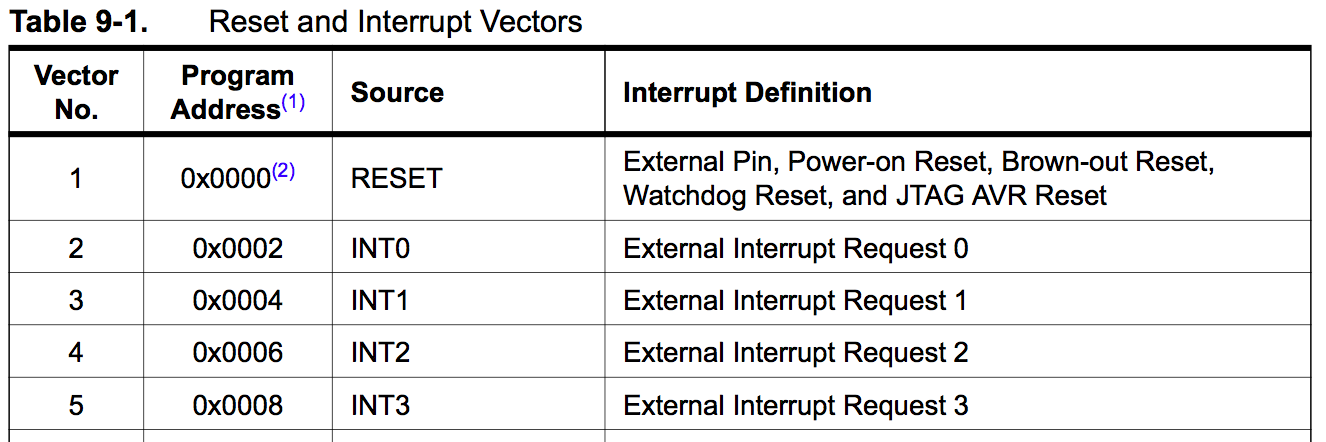
\includegraphics[width=0.95 \linewidth]{../common/images/exampleInterruptVectorAVR.png}
    \caption{First entries in the interrupt Vector for the Atmel AVR® \emph{Source Atmel}}
    \label{fig:itAVR}
  \end{center}
\end{figure}
In our description, we use the \texttt{program address} as the \texttt{trapId} to differentiate interrupt sources.

The description of the interrupt controller is:
\begin{lstlisting}
  void hardInterruptHandler(u32 trapId) {
    if CCR.I then -- global mask    
      -- push current PC: no information about the way PC is stored (same as CALL)
      sram.push(PC{8..1})  --as PC is on 17 bits
      sram.push(PC{16..9})
      -- then branch.
      Fetcher.absBranch((s16)(trapId))
    end if
  }
\end{lstlisting}
It first checks that the global interrupt mask is set (the local mask should be tested before). Then it pushes the program counter (PC) and branches to the appropriate interrupt vector entry. This entry should be a jump instruction to the software interrupt handler. 

There is an example of \emph{timer} using interrupts in chapter \ref{chap:peripherals}.


WARNING: This approach does NOT differ interrupts! In this description, if CCR.I is not set, the interrupt WON'T occur.
%!TEX root = ./main.tex
%!TEX encoding = UTF-8 Unicode

\chapter{Peripherals}
\label{chap:peripherals}
\section{Introduction}
At this date, only few description construction are available to describe peripherals. The 2 constructs are:
\begin{itemize}
\item react to a \emph{read/write access to the memory}. This is useful to describe a basic serial interface for instance.
\item periodic behaviors. This is useful to describe basic timers.
\end{itemize}

\section{Detecting read/write accesses to the memory}
\label{sec:whenReadWrite}
Thanks to \emph{actions}, the user can attach an implementation chunk to a read/write access. The description is inside a component and looks like this:
\begin{lstlisting}
  when [write|read] on <registerName> do
    <implementation>
  end when
\end{lstlisting}
Where:
\begin{itemize}
\item \texttt{[write|read]} is \texttt{read} or \texttt{write};
\item \texttt{<registerName>} is the name of a register (defined either in a component or a memory chunk);
\item\texttt{ <implementation>} is an implementation part, as in methods or behavior in \Blocdo (see section \ref{sec:behDo});
\end{itemize}

Note that this implementation is based on \emph{actions}, and the compilation flag (see section \ref{sec:cflags}) SHOULD be set. If not, the implementation is \emph{never} executed and the simulator does not return any error.

Here is an example of a \emph{dummy} serial line for the AVR:
\begin{lstlisting}
component uart {
  void reset() {
    UCSR0A.UDRE0 := 1 -- transmission complete.
  }

  when write on UDR0 do
    print UDR0
    UCSR0A.UDRE0 := 1 -- transmission complete.
  end when
}
\end{lstlisting}
UDR0 and UCSR0A are Specific Function Registers.

\section{Cyclic behavior}
The following construct models cyclic behaviors:
\begin{lstlisting}
every <unsigned number> cycle [if <condition>] do
  <implementation>
end every
\end{lstlisting}
The code in <implementation> is "executed" periodically, depending on the number of cycles.

Note that:
\begin{itemize}
\item this implementation is based on the \emph{cycles} and can not be used with a functional simulator (the number of cycles stays to 0);
\item the period is defined as an <unsigned number> and \emph{can not} be modified at this date;
\item if the \texttt{[if <condition>]} part is omitted, it is the an always true condition;
\end{itemize}

As for read/write accesses, a cyclic behaviors is described inside a component.

When using the basic temporal description (chapter \ref{chap:timing}), the number of cycles required by an instruction may lead to miss the deadline: if date is 10 and the next instruction requires 3 cycles. Then, even if the cyclic deadline is 12, it will be wake up at date 13. However, the delay is not propagated and the next deadline will be 24.

\emph{This mechanism is not yet implemented in temporal simulators based on the micro-architecture description.}

\subsection{Example}
Here is the example of a simple timer, associated to an interrupt. 

\begin{lstlisting}
component timer2 {
  every 1024 cycle if (TCCR2A.CS2 != 0) do
    TCNT2 := (u8)(TCNT2 + 1) -- FF to 0 is ok (u8)
    if TCNT2 = 0 then      -- overflow
      if TIMSK2.TOIE2 then   -- local interrupt overflow mask
        interrupt \x14
      end if
    end if
  end every
}
\end{lstlisting}

Where registers (TCNT2, TIMSK2 and TCCR2A), are defined like this:
\begin{lstlisting}
component sram {
  memory ram {
    width   := 16  -- get 16 bits / access
    address := \x0..\x10FF
    type    := RAM
    -- ...
    -- timer 2
    register u8  TCCR2A maps to \xB0 {
      CS2 := slice{2..0} -- Clock select bits
    }
    register u8 TCNT2 maps to \xB2
    register u8 TIMSK2 maps to \x70 {
      TOIE2 := slice{0}  -- interrupt enable.
    }
  }
}
\end{lstlisting}
\subsection{Implementation}
The implementation of these cyclic parts uses an ordered single linked list, where the first item has the next deadline. This way, the overhead at runtime (except the execution of the cyclic behavior) is limited to a comparison in the simulator main loop, not depending on the number of cyclic sections.

\subsection{Cyclic behavior on functional simulators}
If there is no temporal description of the processor model, you can use the following work-around at the end of description:
\begin{lstlisting}
timing allInstruction
  do add 1 cycle end do
end timing
\end{lstlisting}
This little description (defined in chapter \ref{chap:timing}) defines that each instruction requires 1 cycle. This simple model allows to use cyclic behaviors, even if the complex temporal model is not yet available.

%\part{Description of the micro-architecture}
%%!TEX root = ./main.tex
%!TEX encoding = UTF-8 Unicode
\chapter{Description de la micro-architecture}
\section{Introduction}
La description de la micro architecture est nécessaire pour la génération d'un simulateur précis (en anglais "Cycle-Accurate Simulator" : CAS). La description d'un pipeline constitue l'élément de base de la micro-architecture dans les processeurs modernes.

\lstset{language=Harmless}
\begin{lstlisting}
architecture Generic {
  device gpr : GPR {
      read is read8 | read16
      write is write8 | write16
      port rs : read (3);
      port rd : write (2);
    }

  device alu : ALU {
      port all;
    }

  device MEM : mem {
      read is read8 | read16
      write is write8 | write16
      shared port fetch : read;
      shared port loadStore : read or write;
    }

  device fetcher : Fetcher {
      port branch : branch;
    }
}
\end{lstlisting}


\appendix
%%!TEX root = ./main.tex
%!TEX encoding = UTF-8 Unicode
\chapter{GDB interface}
\section{Introduction}
\h{} offers three ways of acting on the simulator : two APIs (C and Python) and
the GDB interface. The interface allows to use any tool that have been built on
GDB : IDE integration (eclipse) and GUI like {\tt ddd} for example.

When built for GDB, the simulator acts like a GDB server on which any GDB client
(intended for your target) can connect. The simulated program can be debugged as
any program.

In order to use the GDB interface, two things are needed :
\begin{itemize}
	\item a modified description to include GDB specific informations.
	\item a version of GDB compiled to target the described platform.
\end{itemize}

\section{GDB interface description}
The GDB specific informations are gathered in a component (see section
\ref{sec:component}). The default component must be modified to specify
which component is the GDB component : use the {\tt debug} attribute.
\begin{lstlisting}
	 debug := avrgdb
\end{lstlisting}

This component must have five methods :
\begin{lstlisting}
  u8 read8(u32 v_addr)
  void write8(u32 v_addr, u8 val)
  u8 getNBRegister()
  u32 getRegister(u8 id, out u8 sizeInBits)
  void setRegister(u8 id, u32 value)
\end{lstlisting}

Between the client and the server, GDB uses a protocol called Remote Serial
Protocol\footnote{\url{http://sourceware.org/gdb/current/onlinedocs/gdb_37.html\#SEC673}}.
It specify how data and instructions are transfered between the server and the
client. Registers are identified by a number and memories are mapped in only one
memory space. These methods link this protocol and the description and are
called by the code imitating the GDB server.

\begin{lstlisting}
  u8 read8(u32 v_addr)
\end{lstlisting}
This method has a "virtual" address as input and return the value contained at
this address. The virtual address is used by GDB to differentiate the memories
(RAM,ROM) which may have the same absolute address (on Harvard architecture for
example).
The GDB command {\tt info mem} may give the informations to write this method.

\begin{lstlisting}
  void write8(u32 v_addr, u8 val)
\end{lstlisting}
This method write {\tt val} at {\tt v\_addr} address. For example, in the AVR
model, the addresses below {\tt 0x8000000} are in the RAM, and over {\tt
0x8000000} are in the ROM.
The GDB command {\tt info mem} may give the informations to write this method.

\begin{lstlisting}
  u8 getNBRegister()
  u32 getRegister(u8 id, out u8 sizeInBits)
  void setRegister(u8 id, u32 value)
\end{lstlisting}

These methods are used by the GDB server to get/modify registers value in its order.
{\tt getNBRegister()} returns the number of register that are
transmitted between GDB client and server.
{\tt getRegister()} take an register number as
input {\tt id}, returns the value of the register and set
{\tt sizeInBits} to the value that is required by the
client. {\tt setRegister()} sets the register
{\tt id} to {\tt value}. For all these methods, the register number
is the number of the register in the order defined for the protocol between
client and server.

Some informations about these numbers may be found in  GDB sources. For the PPC
model : {\tt gdb/regformats/reg-ppc.dat} and for the AVR  model {\tt
gdb/avr-tdep.c}. The GDB command {\tt info register} or {\tt info all-registers}
may also give some useful informations on registers order and size. In order to
debug the GDB server, it can be build with the {\tt DEBUG} defined, it will dump
all the communication between client and server. For an example, look at the PPC
or AVR model in the SVN of Harmless.

\section{Short introduction to remote debugging on the simulator}

First, generate the sources and compile the GDB interface, with {\tt make gdb}.

Then launch the GDB server with {\tt <model\_name>\_gdb -f <executable> -p
<port>}. The program is started and stopped before the first instruction,
waiting for GDB orders. Then in GDB:
\begin{verbatim}
# Sometimes architecture must be set in GDB
set architecture powerpc:750

target remote :<port> # Connect to the server
info register         # Display the value of common registers
b my_function         # Add a breakpoint in my_function()
c                     # continu the simulation
# ... Simulation breaks at my_function()
bt                    # Display backtrace
print i               # Display the value of the i variable
x 42                  # examine memory at address 42
\end{verbatim}

More information about GDB command, are available in the GDB
manual\footnote{\url{http://sourceware.org/gdb/current/onlinedocs/gdb_4.html\#SEC14}}

%!TEX root = ./main.tex
%!TEX encoding = UTF-8 Unicode
\chapter{Task Scheduling and Stack Safety}
\section{Introduction}
\h\ aim to simulate real-time software, this module offers real-time application analysis. This appendix present how to use mechanism that allows to detect task switch and analyze task's stack (usage and corruption).

\noindent Stack Monitoring offers various informations :
\begin{itemize}
	\item \emph{Task Scheduling : }task activation are detected and a T3 trace file could be generated to visualized application behavior in a gantt diagram. The simulator only need task main function symbol and stack size.
	\item \emph{Stack Monitoring and Safety :} provide a good way to evaluate stack use and detect stack failure (like underflow or overflow). The simulator may need some os system function symbol to exclude them from stack failure detection.
\end{itemize}

\emph{Note} : executable file have to be \emph{ELF files}, it's used to resolve function symbol.
% SECTIONS %
\section{Description modification}


Task monitoring only need a slight modification of \h\ processor description. From \h\ view Task monitoring only need to know which instruction or group of instruction is used to CALL, it also uses Stack Pointer value\footnote{SP register have to be defined (for the time being since no generic way to access stack pointer is provided by current \h\ version) SP() is used to get Stack Pointer value.}.

\begin{verbatim} 
 #SP_Check flag should be added to each CALL type instructions (for all views).
\end{verbatim}

\noindent Example on ARM processor description :
\begin{lstlisting}
syntax branch #branch
  "b"
  select
    case #noLink --nothing
    case #withLink  #SP_Check "l"
...

syntax blx #branch #withLink #SP_Check #Thumb 
  "blx"
...

behavior branchInst #branch
    ..
    case #withLink  #SP_Check
	...
	
behavior branchLinkExchangeInst #branch #withLink #Thumb #SP_Check
...

format blx1 #branch #withLink #Thumb #SP_Check -- branch, link and change ISA to Thumb.
...

format blx2 #branch #withLink #Thumb #SP_Check -- branch, link and change ISA to Thumb.
...
 \end{lstlisting}

% SECTIONS %
\section{Compilation flags}
Stack analysis requires significant amount of computation time, so it's an optional tool for \h\ simulator, some building option are required (modification in generated \texttt{Makefile}).

\subsection{Required build options}
Stack monitoring need \emph{action} mechanism (simulation time increase by about 40\%), so the flag \texttt{GADL\_NO\_ACTION} should NOT be defined (see section \ref{sec:cflags}).

\subsection{Task Scheduling}
\noindent Task Scheduling is activated by following building option (simulation time increases about 10\%).
\begin{verbatim}
DEFINES += -DGADL_SP_CHECK_ALLOWED
\end{verbatim}

\subsection{Stack safety monitoring}
\noindent Stack use and safety monitoring is activated by following options (simulation time increase again by about  3\% in worst case).
\begin{verbatim}
DEFINES += -DGADL_SP_FAILURE_CHECK_ALLOWED 
DEFINES += -DGADL_SP_CHECK_ALLOWED
\end{verbatim}

% SECTIONS %
\section{Task Scheduling}
Stack analysis provides to \h\ tools to detect the scheduling of the tasks, in the context of a multi-tasking system. In a multi-tasking system, each task has its own context (stack and register set), it's used to allow detection any user application modification. This tool provides a Gantt from application execution in order to analyze scheduling.

\subsection{Task declaration}
Each Task of application have to be declared to \h\ generated simulator using following function.

\lstset{language=C++}
\begin{lstlisting}
void addTaskToMonitor(string taskName,string functionSym,u32 size);
\end{lstlisting}
\begin{itemize}
	\item  {\tt taskName} is an arbitrary name to describe Task (ex.  {\tt "MainTask"})
	\item  {\tt functionSym} is Task's main function symbol (ex.  {\tt "function\_of\_task1"}).
	\item  {\tt size}  is size of Task's stack (ex.  {\tt 250} a wrong value will result in a simulation failure).
\end{itemize}
\emph{Note:} Two tasks or more can share the same main function, the tool will automatically detect associated stack.

\subsection{Task data}
\noindent Simulator can display list of Task and associated data using following function :
\begin{lstlisting}
void printTaskList()
 \end{lstlisting}
 
 \begin{verbatim}
********************************
* STACK/TASK List Informations *
********************************

Task n 5 (Task 5) : Fct@0 Stack (size=250) : init@0 -1- StackRealUse=0
Task n 4 (Task 4) : Fct@134 Stack (size=250) : init@58d -1- StackRealUse=0
Task n 3 (Task 3) : Fct@122 Stack (size=250) : init@6fa -1- StackRealUse=0
Task n 2 (Task 2) : Fct@110 Stack (size=20) : init@468 -1- StackRealUse=0
Task n 1 (Task 1) : Fct@ee Stack (size=250) : init@368 -1- StackRealUse=0
\end{verbatim}

 \begin{itemize}
	\item  {\tt Task n ..} specific id of task in simulator (0 is {\tt Unkwnon}, then by order of add)
	\item  {\tt task\_name} is task name add by user
	\item  {\tt Fct@...} address of main function of task (automatically detected)
	\item  {\tt size=...} size of stack add by user
	\item  {\tt init@...}  stack initial address
	\item  {\tt -...-} : {\tt 1} if initial value is detected / {\tt 0} if no initial value is detected
	\item  {\tt StaclRealUse=...} not used in this mode
\end{itemize}

\subsection{Task switch data}
\noindent Simulator can display a list of Task switch and activation using following function. Undeclared task events will be associated to task number 0 {\tt  Unkwnon Task}.
\begin{lstlisting}
void printControllerSwitchList();
\end{lstlisting}

\begin{verbatim}
********************************
*       TASK Switch List       *
********************************
Task n 0 --Running   Date=1 SP@0
Task n 5 --Activate  Date=0 SP@0
Task n 5 --Running   Date=0 SP@0
Task n 0 --Running   Date=12784 SP@10fd
Task n 1 --Activate  Date=16316 SP@368
Task n 1 --Running   Date=16316 SP@368
Task n 2 --Activate  Date=20040 SP@468
Task n 2 --Running   Date=20040 SP@468
\end{verbatim}

 \begin{itemize}
	\item  {\tt Task n ..} specific id of task in simulator (0 is {\tt Unkwnon}, then by order of add)
	\item {\tt --.......}  {\tt Running} : stack is in task stack /   {\tt Activate} : task function called
	\item  {\tt Date=...} date in processor cycle (from simulator)
	\item  {\tt SP@... } Stack Pointer value when event occured
\end{itemize}

\subsection{T3 trace generation (Gantt)}
T3\footnote{\url{http://jttrace.rts-software.org} provides a good way to visualize application execution using a Gantt. The simulator can generate a T3} compatible file in order to display a Gantt from application.
\begin{lstlisting}
void writeTraceT3(string path);
\end{lstlisting}
T3 {\tt Idle Task} (maximum ID in T3) is used as {\tt Unknown task} (null ID in \h\ )
\begin{itemize}
	\item  {\tt path} path and name of target file (ex  {\tt "./trace.txt"})
\end{itemize}




% SECTIONS %
\section{Stack Use and Safety Monitoring}
Stack analysis provided tools to find an appropriate stack size by analyzing real stack use of each declared task and detecting failure.

\subsection{Size of stack protection area}
User can choose how much byte upper and lower from the stack area will be associated to failure detection. 
\lstset{language=C++}
\begin{lstlisting}
void setSizeOfStackProtectionArea(type_sp size);
\end{lstlisting}
 \begin{itemize}
	\item  {\tt size} : size of upper and lower protection area used to detect stack failure. TODO dessin!!
\end{itemize}

\subsection{System function exclusion}
Context switch function can be detected as stack failure where there is only a normal behavior of OS, those function can be exclused using following function
\lstset{language=C++}
\begin{lstlisting}
void setExclusionOnSystFunction(string symbol);
\end{lstlisting}
 \begin{itemize}
	\item  {\tt symbol} :  a system function (wich need to be excluded) symbol  (ex  {\tt "tpl\_put\_preempted\_proc"})
\end{itemize}

\subsection{Stack failure message}
Any stack failure detected will automatically be noticed by the simulator providing program adress where it ocured for debugging purpose.

\begin{verbatim}
ERROR in task n 2 (Task 2) @15ac STACK OVERFLOW
ERROR in task n 2 (Task 2) @15ae STACK OVERFLOW
\end{verbatim}

 \begin{itemize}
	\item  {\tt task n ..} : specific id of task in simulator
	\item {\tt taskName} : name of task defined by user
	\item  {\tt @...} : program address where failure occured
	\item  {\tt STACK ...... } : {\tt OVERFLOW} or {\tt UNDERFLOW}
\end{itemize}

\subsection{Stack use print}
\noindent Simulator can display stack's use, using following function :
\begin{lstlisting}
void printTaskList();
 \end{lstlisting}
 
 \begin{verbatim}
********************************
* STACK/TASK List Informations *
********************************

Task n 4 (Task 4) : Fct@134 Stack (size=250) : init@58d -1- StackRealUse=22
Task n 3 (Task 3) : Fct@122 Stack (size=250) : init@6fa -1- StackRealUse=22
Task n 2 (Task 2) : Fct@110 Stack (size=20) : init@468 -1- StackRealUse=19 !! Overflow !!  at PC@15ac
Task n 1 (Task 1) : Fct@ee Stack (size=250) : init@368 -1- StackRealUse=47
\end{verbatim}

 \begin{itemize}
	\item  cf. task scheduling
	\item  {\tt StaclRealUse=...} is the maximum real stack use detected by stack analysis tool
	\item {\tt !! Overflow !! at PC@...} program address of first stack failure
\end{itemize}
 
 % SECTIONS %
\section{Short example of application}
Example included four task, one posses a too small stack to test stack failure dectetion, executable file have to be \emph{ELF files}.
\subsection{Python Script}
Simulator is build with all Stack Analysis options.
\lstset{language=python}
\begin{lstlisting}
#!/usr/bin/python
import sys

# Looks in AT90CAN128 directory to find the processor arch
sys.path.append("./AT90CAN128")
# Provide simulator
from AT90CAN128 import arch	
# Need to access Stack Tools
from AT90CAN128 import stackSpyController

# Create simulator 
f=arch()
# Read executable file (ELF files only)
f.readCodeFile("./AVRTrampolineBinTest1")					

# Get an access to Stack Tools
stackCtrl=f.getStackSpyController()				

# Declaration of Exclusion function for Stack Failure detection
stackCtrl.setExclusionOnSystFunction("tpl_put_preempted_proc");

# Declaration of Tasks in simulator
stackCtrl.addTaskToMonitor("Task 1","startTask_function",250);
stackCtrl.addTaskToMonitor("Task 2","secondTask_function",20);
stackCtrl.addTaskToMonitor("Task 3","thirdTask_function",250);
stackCtrl.addTaskToMonitor("Task 4","fourthTask_function",250);

print "-- task's switching and stack usage analysis --"
f.execInst(10000000) #run until breakpoint

# Print Task data (including real task uses and failure)
print ">> Task List"
stackCtrl.printTaskList();

#Print Task events (activation and switch)
print ">> Switch List"
stackCtrl.printControllerSwitchList()

# Write a T3 file to visualize the Gantt of Task Scheduling
stackCtrl.writeTraceT3("trace.txt");
\end{lstlisting}

\subsection{Result of Simulation}

\begin{verbatim}
$ ./test_stack.py 
-- task's switching and stack usage analysis --
ERROR in task n 2 (Task 2) @15ac STACK OVERFLOW
ERROR in task n 2 (Task 2) @15ae STACK OVERFLOW
>> Task List

********************************
* STACK/TASK List Informations *
********************************

Task n 4 (Task 4) : Fct@134 Stack (size=250) : init@58d -1- StackRealUse=22
Task n 3 (Task 3) : Fct@122 Stack (size=250) : init@6fa -1- StackRealUse=22
Task n 2 (Task 2) : Fct@110 Stack (size=20) : init@468 -1- StackRealUse=19 !! Overflow !!  at PC@15ac
Task n 1 (Task 1) : Fct@ee Stack (size=250) : init@368 -1- StackRealUse=47

>> Switch List

********************************
*       TASK Switch List       *
********************************

Task n 0 --Running   Date=1 SP@0
Task n 1 --Activate  Date=16316 SP@368
Task n 1 --Running   Date=16316 SP@368
Task n 2 --Activate  Date=20040 SP@468
Task n 2 --Running   Date=20040 SP@468
Task n 1 --Running   Date=21222 SP@359
Task n 3 --Activate  Date=25010 SP@6fa
Task n 3 --Running   Date=25010 SP@6fa
Task n 1 --Running   Date=26192 SP@359
Task n 4 --Activate  Date=30012 SP@58d
Task n 4 --Running   Date=30012 SP@58d
Task n 1 --Running   Date=31194 SP@359
\end{verbatim}

\subsection{T3 Gantt from Simulation}

 \begin{itemize}
	\item {\tt  idlle} : is {\tt Unknown task}
	\item  {\tt Task n 0} is the main task (Task 1)
\end{itemize}

 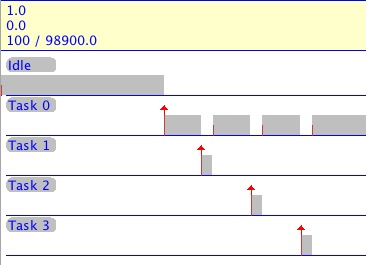
\includegraphics[width=0.8 \linewidth]{../common/images/appendixBSExampleStackAnalysisGantt.jpg}



\end{document}
